% ============================================================================
% C⁴ / deppy — 200 Beamer Slides for a PL Beginner
% ============================================================================
\documentclass[aspectratio=169,11pt]{beamer}

\usetheme{Madrid}
\usecolortheme{seahorse}
\setbeamertemplate{navigation symbols}{}
\setbeamertemplate{footline}[frame number]

% ── Packages ──────────────────────────────────────────────────────────────
\usepackage{amsmath,amssymb,amsthm}
\usepackage{stmaryrd}
\usepackage{mathtools}
\usepackage{tikz}
\usetikzlibrary{arrows.meta,positioning,calc,decorations.pathmorphing,
  shapes.geometric,fit,backgrounds}
\usepackage{listings}
\usepackage{xcolor}
\usepackage{booktabs}
\usepackage{graphicx}
\usepackage{hyperref}

% ── Colors ────────────────────────────────────────────────────────────────
\definecolor{codegreen}{rgb}{0.2,0.6,0.2}
\definecolor{codepurple}{rgb}{0.58,0,0.82}
\definecolor{codeblue}{rgb}{0.1,0.3,0.7}
\definecolor{codered}{rgb}{0.8,0.1,0.1}
\definecolor{codegray}{rgb}{0.5,0.5,0.5}
\definecolor{backgray}{rgb}{0.97,0.97,0.97}
\definecolor{trustgreen}{rgb}{0.0,0.6,0.0}
\definecolor{trustyellow}{rgb}{0.8,0.6,0.0}
\definecolor{trustred}{rgb}{0.8,0.0,0.0}

% ── Listings ──────────────────────────────────────────────────────────────
\lstset{
  basicstyle=\ttfamily\scriptsize,
  keywordstyle=\color{codeblue}\bfseries,
  stringstyle=\color{codered},
  commentstyle=\color{codegreen}\itshape,
  numberstyle=\tiny\color{codegray},
  breaklines=true,
  backgroundcolor=\color{backgray},
  frame=single,
  framerule=0.3pt,
  numbers=left,
  numbersep=5pt,
  showstringspaces=false,
  tabsize=2,
}
\lstdefinelanguage{deppy}{
  morekeywords={def,return,if,else,for,while,import,from,class,
    guarantee,spec,hole,assume,check,given,True,False,None,
    lambda,and,or,not,in,is,as,with,try,except,raise,yield},
  sensitive=true,
  morecomment=[l]{\#},
  morestring=[b]",
  morestring=[b]',
}

% ── Math macros ───────────────────────────────────────────────────────────
\newcommand{\Cfour}{\mathrm{C}^4}
\newcommand{\CCTT}{\mathrm{CCTT}}
\newcommand{\CIC}{\mathrm{CIC}}
\newcommand{\Path}{\mathsf{Path}}
\newcommand{\PyObj}{\mathsf{PyObj}}
\newcommand{\OTerm}{\mathsf{OTerm}}
\newcommand{\interval}{\mathbb{I}}
\newcommand{\Hone}{H^1}
\newcommand{\Htwo}{H^2}
\newcommand{\Hzero}{H^0}
\newcommand{\site}{\mathcal{S}}
\newcommand{\restr}[2]{#1|_{#2}}
\newcommand{\den}[1]{\llbracket #1 \rrbracket}
\newcommand{\covers}{\mathcal{U}}
\newcommand{\transp}{\mathsf{transp}}
\newcommand{\desc}{\mathsf{desc}}


\title{\textbf{deppy \& $\Cfour$} \\[6pt]
  \large Cohomological Type Theory for Verified Python}
\subtitle{A Gentle Introduction for PL Beginners}
\author{The deppy Project}
\date{2026}

\begin{document}

% ══════════════════════════════════════════════════════════════════════════
% PART 0: TITLE AND OVERVIEW (Slides 1–10)
% ══════════════════════════════════════════════════════════════════════════

% --- Slide 1 ---
\begin{frame}
\titlepage
\end{frame}

% --- Slide 2 ---
\begin{frame}{What This Talk Is About}
\begin{itemize}
\item \textbf{Goal}: Automatically verify that Python programs are correct
\item \textbf{Tool}: \texttt{deppy} --- a hybrid type system for Python
\item \textbf{Theory}: $\Cfour$ --- a new type theory that combines
  \begin{itemize}
  \item Dependent types (like Lean, Coq, Agda)
  \item Algebraic geometry (sheaves, cohomology)
  \item Cubical type theory (paths, univalence)
  \end{itemize}
\item \textbf{Audience}: You! A PL student seeing these ideas for the first time
\end{itemize}
\end{frame}

% --- Slide 3 ---
\begin{frame}{Why Should You Care?}
\begin{columns}
\begin{column}{0.5\textwidth}
\textbf{The Problem:}
\begin{itemize}
\item Software has bugs
\item Testing catches \emph{some} bugs
\item But testing can't prove \emph{absence} of bugs
\item Critical systems need \emph{guarantees}
\end{itemize}
\end{column}
\begin{column}{0.5\textwidth}
\textbf{The Dream:}
\begin{itemize}
\item Write Python code normally
\item Annotate what it \emph{should} do
\item A tool \emph{proves} it does that
\item No false positives, no sampling
\end{itemize}
\end{column}
\end{columns}
\end{frame}

% --- Slide 4 ---
\begin{frame}{Roadmap}
\begin{enumerate}
\item \textbf{Part I}: What is program equivalence? (Slides 11--40)
\item \textbf{Part II}: Types and dependent types (Slides 41--70)
\item \textbf{Part III}: Sheaves and cohomology for programs (Slides 71--110)
\item \textbf{Part IV}: The $\Cfour$ calculus (Slides 111--150)
\item \textbf{Part V}: deppy in practice (Slides 151--180)
\item \textbf{Part VI}: Metatheory and comparison (Slides 181--200)
\end{enumerate}
\end{frame}

% --- Slide 5 ---
\begin{frame}{What Is deppy?}
\begin{center}
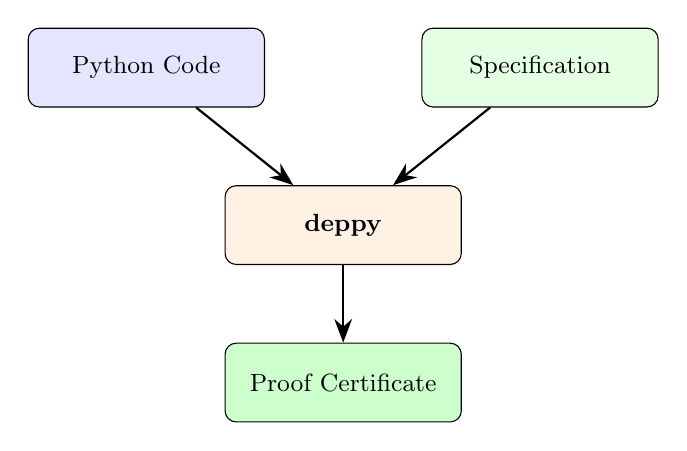
\begin{tikzpicture}[
  box/.style={draw, rounded corners, minimum width=3cm, minimum height=1cm,
    fill=blue!10, font=\small},
  arr/.style={-{Stealth[length=3mm]}, thick}
]
\node[box] (py) at (0,0) {Python Code};
\node[box, fill=green!10] (spec) at (5,0) {Specification};
\node[box, fill=orange!10] (deppy) at (2.5,-2) {\textbf{deppy}};
\node[box, fill=green!20] (proof) at (2.5,-4) {Proof Certificate};
\draw[arr] (py) -- (deppy);
\draw[arr] (spec) -- (deppy);
\draw[arr] (deppy) -- (proof);
\end{tikzpicture}
\end{center}

deppy takes your Python code + a specification and produces a
\textbf{machine-checked proof} that the code satisfies the spec.
\end{frame}

% --- Slide 6 ---
\begin{frame}[fragile]{A First Example}
\begin{lstlisting}[language=deppy]
from deppy.hybrid import guarantee

@guarantee("returns a sorted list")
def my_sort(lst):
    # Bubble sort
    a = list(lst)
    for i in range(len(a)):
        for j in range(len(a) - i - 1):
            if a[j] > a[j+1]:
                a[j], a[j+1] = a[j+1], a[j]
    return a
\end{lstlisting}

\vspace{0.5em}
The \lstinline|@guarantee| decorator tells deppy: ``prove that the return
value is always sorted.'' deppy does the rest.
\end{frame}

% --- Slide 7 ---
\begin{frame}{How deppy Verifies}
\begin{enumerate}
\item \textbf{Parse} the Python code into an abstract syntax tree (AST)
\item \textbf{Compile} the AST into a mathematical object called an \textbf{OTerm}
\item \textbf{Decompose} the specification into checkable predicates
\item \textbf{Prove} each predicate using Z3 (SMT solver) or sheaf descent
\item \textbf{Certify} the result with a trust level
\end{enumerate}

\vspace{1em}
\begin{center}
\begin{tabular}{ll}
\toprule
\textbf{Trust Level} & \textbf{Meaning} \\
\midrule
\textcolor{trustgreen}{LEAN\_VERIFIED} & Machine-checked Lean proof \\
\textcolor{trustgreen}{Z3\_PROVEN} & SMT solver proved it \\
\textcolor{trustyellow}{LLM\_JUDGED} & AI oracle says correct \\
\textcolor{trustred}{UNTRUSTED} & No verification yet \\
\bottomrule
\end{tabular}
\end{center}
\end{frame}

% --- Slide 8 ---
\begin{frame}{What Is $\Cfour$?}
\begin{block}{Cohomological Calculus of Constructions}
$\Cfour$ is a \textbf{dependent type theory} that extends the Calculus of
Inductive Constructions (CIC, the kernel of Lean and Coq) with:

\begin{itemize}
\item \textbf{Site-decorated universes} --- types are fibered over a site
\item \textbf{Cubical path types} --- equalities are paths in a space
\item \textbf{Descent rule} --- local proofs glue into global proofs
\item \textbf{Mathlib import} --- use any of 177,000+ Lean theorems
\item \textbf{OTerm embedding} --- Python programs are first-class types
\end{itemize}
\end{block}
\end{frame}

% --- Slide 9 ---
\begin{frame}{The Key Insight}
\begin{center}
\Large
\textbf{Bugs are cohomology classes.}
\end{center}

\vspace{1em}
\begin{itemize}
\item A program works correctly on each ``type fiber'' (ints, strings, lists)
\item But it might fail when fibers \emph{interact}
\item The \emph{obstruction} to gluing local correctness into global
  correctness lives in $\Hone$
\item $\Hone = 0$ means: \textbf{no bugs} (local correctness implies global)
\item $\Hone \neq 0$ means: there's a \textbf{cohomological bug}
\end{itemize}
\end{frame}

% --- Slide 10 ---
\begin{frame}{Prerequisites}
\textbf{What you need to know:}
\begin{itemize}
\item Basic Python programming
\item What a function is, what types are
\item Comfortable with mathematical notation
\end{itemize}

\vspace{1em}
\textbf{What we'll teach you:}
\begin{itemize}
\item Dependent types (from scratch)
\item Sheaves and cohomology (intuition first, formalism later)
\item How all of this helps verify real programs
\end{itemize}
\end{frame}


% ══════════════════════════════════════════════════════════════════════════
% PART I: PROGRAM EQUIVALENCE (Slides 11–40)
% ══════════════════════════════════════════════════════════════════════════

\part{Program Equivalence}

% --- Slide 11 ---
\begin{frame}{Part I: Program Equivalence}
\begin{center}
\Huge \textbf{When are two programs ``the same''?}
\end{center}
\end{frame}

% --- Slide 12 ---
\begin{frame}[fragile]{Two Sorting Algorithms}
\begin{columns}
\begin{column}{0.48\textwidth}
\begin{lstlisting}[language=deppy,title={\textbf{Bubble Sort}}]
def sort_a(lst):
    a = list(lst)
    for i in range(len(a)):
        for j in range(len(a)-i-1):
            if a[j] > a[j+1]:
                a[j], a[j+1] = a[j+1], a[j]
    return a
\end{lstlisting}
\end{column}
\begin{column}{0.48\textwidth}
\begin{lstlisting}[language=deppy,title={\textbf{Selection Sort}}]
def sort_b(lst):
    a = list(lst)
    for i in range(len(a)):
        m = i
        for j in range(i+1, len(a)):
            if a[j] < a[m]:
                m = j
        a[i], a[m] = a[m], a[i]
    return a
\end{lstlisting}
\end{column}
\end{columns}

\vspace{1em}
\textbf{Question}: Are these ``the same'' program?

\textbf{Answer}: They look different, but they compute the same
function: $\mathtt{sort\_a}(x) = \mathtt{sort\_b}(x)$ for all lists $x$.
\end{frame}

% --- Slide 13 ---
\begin{frame}{What Does ``Same'' Mean?}
\begin{block}{Extensional Equivalence}
Two functions $f$ and $g$ are \textbf{extensionally equivalent} if:
\[
  \forall x.\; f(x) = g(x)
\]
They produce the same output on every input.
\end{block}

\vspace{0.5em}
\begin{itemize}
\item We don't care \emph{how} they compute --- only \emph{what} they compute
\item Bubble sort and selection sort are equivalent in this sense
\item This is the gold standard for program correctness
\end{itemize}
\end{frame}

% --- Slide 14 ---
\begin{frame}{Why Is Equivalence Hard?}
\begin{itemize}
\item \textbf{Rice's theorem}: Every non-trivial semantic property of programs
  is undecidable
\item Translation: No algorithm can always correctly decide if $f \equiv g$
\item \textbf{But}:
  \begin{itemize}
  \item We can decide \emph{many} cases in practice
  \item We can use structured mathematical reasoning
  \item We can decompose the problem into manageable pieces
  \end{itemize}
\end{itemize}

\vspace{0.5em}
\begin{block}{The deppy approach}
Don't try to solve the general halting problem.
Instead, use \textbf{algebraic structure} to handle the cases that
matter for real code.
\end{block}
\end{frame}

% --- Slide 15 ---
\begin{frame}[fragile]{Approach 1: Testing}
\begin{lstlisting}[language=deppy]
# Does sort_a == sort_b?
for test_input in [[3,1,2], [1], [], [5,4,3,2,1], ...]:
    assert sort_a(test_input) == sort_b(test_input)
print("All tests passed!")
\end{lstlisting}

\vspace{1em}
\textbf{Pros}: Easy, fast, catches obvious bugs

\textbf{Cons}:
\begin{itemize}
\item Can only test \emph{finitely many} inputs
\item Might miss edge cases (empty list? negative numbers? huge lists?)
\item ``Program testing can be used to show the presence of bugs,
  but never to show their absence'' --- Dijkstra
\end{itemize}
\end{frame}

% --- Slide 16 ---
\begin{frame}{Approach 2: Formal Verification}
\textbf{Idea}: Write a \emph{mathematical proof} that $f \equiv g$.

\vspace{0.5em}
\textbf{Tools that exist:}
\begin{description}
\item[Lean/Coq] Write proofs in a proof assistant. Very powerful,
  but requires learning a new language and writing proofs by hand.
\item[Z3/SMT] Encode the problem as a logic formula and let a solver
  decide. Automated, but limited to certain theories (linear arithmetic,
  arrays, bitvectors).
\item[Model checking] Enumerate all states. Works for finite systems,
  but state explosion for real programs.
\end{description}

\vspace{0.5em}
\textbf{None of these work well for arbitrary Python programs.}

That's where deppy comes in.
\end{frame}

% --- Slide 17 ---
\begin{frame}{Approach 3: deppy's Strategy}
\begin{enumerate}
\item \textbf{Compile} both programs to OTerms (denotational semantics)
\item \textbf{Decompose} by input type (integers, strings, lists, \ldots)
\item \textbf{Prove} equivalence on each type ``fiber'' using Z3
\item \textbf{Glue} the per-fiber proofs using cohomology
\item \textbf{Report}: Equivalent? Yes/No, with proof certificate
\end{enumerate}

\begin{center}
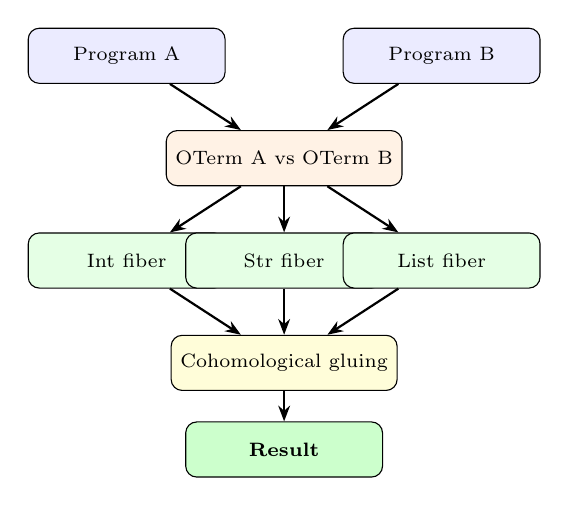
\begin{tikzpicture}[
  box/.style={draw, rounded corners, minimum width=2.5cm, minimum height=0.7cm,
    fill=blue!8, font=\scriptsize},
  arr/.style={-{Stealth[length=2mm]}, thick}
]
\node[box] (a) at (0,0) {Program A};
\node[box] (b) at (4,0) {Program B};
\node[box, fill=orange!10] (ot) at (2,-1.3) {OTerm A vs OTerm B};
\node[box, fill=green!10] (f1) at (0,-2.6) {Int fiber};
\node[box, fill=green!10] (f2) at (2,-2.6) {Str fiber};
\node[box, fill=green!10] (f3) at (4,-2.6) {List fiber};
\node[box, fill=yellow!15] (glue) at (2,-3.9) {Cohomological gluing};
\node[box, fill=green!20] (res) at (2,-5.0) {\textbf{Result}};
\draw[arr] (a) -- (ot);
\draw[arr] (b) -- (ot);
\draw[arr] (ot) -- (f1);
\draw[arr] (ot) -- (f2);
\draw[arr] (ot) -- (f3);
\draw[arr] (f1) -- (glue);
\draw[arr] (f2) -- (glue);
\draw[arr] (f3) -- (glue);
\draw[arr] (glue) -- (res);
\end{tikzpicture}
\end{center}
\end{frame}

% --- Slide 18 ---
\begin{frame}{What Is an OTerm?}
\begin{block}{Definition (Informal)}
An \textbf{OTerm} is a mathematical representation of what a Python
expression \emph{computes}, stripped of all implementation details.
\end{block}

\vspace{0.5em}
Think of it like this:
\begin{itemize}
\item Python code: \texttt{x + y} $\longrightarrow$ OTerm: $\mathsf{OOp}(+, [x, y])$
\item Python code: \texttt{42} $\longrightarrow$ OTerm: $\mathsf{OLit}(42)$
\item Python code: \texttt{sum(lst)} $\longrightarrow$ OTerm: $\mathsf{OFold}(+, 0, \mathit{lst})$
\end{itemize}

\vspace{0.5em}
OTerms are the ``mathematical soul'' of a program --- two programs
that compute the same thing have equivalent OTerms.
\end{frame}

% --- Slide 19 ---
\begin{frame}{OTerm Constructors}
\begin{center}
\begin{tabular}{lll}
\toprule
\textbf{Constructor} & \textbf{Meaning} & \textbf{Python Example} \\
\midrule
$\mathsf{OVar}(x)$ & Variable & \texttt{x} \\
$\mathsf{OLit}(v)$ & Literal value & \texttt{42}, \texttt{"hello"} \\
$\mathsf{OOp}(\diamond, [a,b])$ & Binary operation & \texttt{a + b} \\
$\mathsf{OFold}(\diamond, e, xs)$ & Fold/reduce & \texttt{sum(xs)} \\
$\mathsf{OCase}(c, t, f)$ & Conditional & \texttt{t if c else f} \\
$\mathsf{OApp}(f, x)$ & Function call & \texttt{f(x)} \\
$\mathsf{OFix}(n, b)$ & Recursion & \texttt{def n: ... n(...)} \\
$\mathsf{OComp}(e, x, s)$ & Comprehension & \texttt{[e for x in s]} \\
\bottomrule
\end{tabular}
\end{center}

These 13 constructors can represent any Python computation.
\end{frame}

% --- Slide 20 ---
\begin{frame}[fragile]{From Python to OTerm: An Example}
\begin{lstlisting}[language=deppy]
def sum_list(lst):
    total = 0
    for x in lst:
        total += x
    return total
\end{lstlisting}

\vspace{0.5em}
$\Downarrow$ \textbf{Compilation to OTerm}

\[
  \den{\mathtt{sum\_list}} = \mathsf{OFold}(+,\; \mathsf{OLit}(0),\; \mathsf{OVar}(\mathit{lst}))
\]

\vspace{0.5em}
The loop-based accumulation pattern is recognized as a \textbf{fold}.
This is the same OTerm you'd get from \texttt{sum(lst)} or
\texttt{functools.reduce(operator.add, lst, 0)}.
\end{frame}

% --- Slide 21 ---
\begin{frame}{The 24 Dichotomies}
OTerms obey \textbf{algebraic laws} called \textbf{dichotomies} (D1--D24):

\vspace{0.5em}
\begin{columns}
\begin{column}{0.48\textwidth}
\begin{description}
\item[D1] $a + b \equiv b + a$ \\ (addition commutes)
\item[D2] $(a + b) + c \equiv a + (b + c)$ \\ (addition associates)
\item[D3] $a + 0 \equiv a$ \\ (zero is identity)
\item[D7] $a \cdot 1 \equiv a$ \\ (one is mult.\ identity)
\item[D10] $\text{if True then } a \text{ else } b \equiv a$
\end{description}
\end{column}
\begin{column}{0.48\textwidth}
\begin{description}
\item[D14] $\mathsf{fold}(+, 0, []) \equiv 0$
\item[D16] $\text{len}(\text{append}(l,x)) \equiv \text{len}(l) + 1$
\item[D20] Same spec $\Rightarrow$ equivalent
\item[D22] map-fold fusion
\item[D24] Sort is idempotent
\end{description}
\end{column}
\end{columns}

\vspace{0.5em}
These are the ``axioms of Python computation'' --- every equivalence
we prove is ultimately a chain of dichotomy applications.
\end{frame}

% --- Slide 22 ---
\begin{frame}{Axiom Chains}
To prove $f \equiv g$, we find a sequence of dichotomy rewrites:

\[
  \den{f} \xrightarrow{\text{D1}} t_1 \xrightarrow{\text{D14}} t_2
  \xrightarrow{\text{D3}} \cdots \xrightarrow{\text{D7}} \den{g}
\]

\vspace{0.5em}
\begin{block}{Example}
Prove $\mathtt{sum([a,b,c])} \equiv \mathtt{a + b + c}$:
\begin{align*}
  \mathsf{OFold}(+, 0, [a,b,c])
  &\xrightarrow{\text{D14}} \mathsf{OOp}(+, [0, \mathsf{OOp}(+, [a, \mathsf{OOp}(+, [b,c])])])
  \\
  &\xrightarrow{\text{D3}} \mathsf{OOp}(+, [a, \mathsf{OOp}(+, [b,c])])
  \\
  &\xrightarrow{\text{D2}} \mathsf{OOp}(+, [\mathsf{OOp}(+, [a,b]), c])
\end{align*}
\end{block}
\end{frame}

% --- Slide 23 ---
\begin{frame}[fragile]{When Two Programs Are NOT Equivalent}
\begin{columns}
\begin{column}{0.48\textwidth}
\begin{lstlisting}[language=deppy,title={\textbf{Program A}}]
def count(lst, x):
    c = 0
    for item in lst:
        if item == x:
            c += 1
    return c
\end{lstlisting}
\end{column}
\begin{column}{0.48\textwidth}
\begin{lstlisting}[language=deppy,title={\textbf{Program B (buggy)}}]
def count(lst, x):
    c = 0
    for item in lst:
        if item >= x:  # BUG: >= not ==
            c += 1
    return c
\end{lstlisting}
\end{column}
\end{columns}

\vspace{0.5em}
\textbf{Counterexample}: \texttt{count([1,2,3], 2)}
\begin{itemize}
\item Program A returns \texttt{1} (only \texttt{2 == 2})
\item Program B returns \texttt{2} (both \texttt{2 >= 2} and \texttt{3 >= 2})
\end{itemize}
\end{frame}

% --- Slide 24 ---
\begin{frame}{The Challenge of Scale}
\textbf{Real programs} are much bigger than toy examples:

\begin{itemize}
\item Hundreds of lines, multiple functions
\item Complex control flow (nested loops, recursion, exceptions)
\item Multiple input types (ints AND strings AND lists AND dicts)
\item Library calls, side effects, mutable state
\end{itemize}

\vspace{0.5em}
\textbf{Key question}: How do we scale formal verification to handle
real Python?

\textbf{Answer}: \emph{Decomposition}. Break the problem into
independent pieces, verify each piece, then reassemble.

This is exactly what sheaves and cohomology give us.
\end{frame}

% --- Slide 25 ---
\begin{frame}{What Are ``Type Fibers''?}
\begin{block}{Intuition}
A \textbf{type fiber} is the behavior of a function restricted to one
input type.
\end{block}

\vspace{0.5em}
Consider a function \texttt{f(x)} that accepts ints, strings, and lists:
\begin{itemize}
\item \textbf{Int fiber}: How does \texttt{f} behave when \texttt{x} is an int?
\item \textbf{Str fiber}: How does \texttt{f} behave when \texttt{x} is a string?
\item \textbf{List fiber}: How does \texttt{f} behave when \texttt{x} is a list?
\end{itemize}

\vspace{0.5em}
Python's duck typing means a single function can behave very differently
on different types.  Fibers let us analyze each behavior separately.
\end{frame}

% --- Slide 26 ---
\begin{frame}[fragile]{Example: Per-Fiber Analysis}
\begin{lstlisting}[language=deppy]
def double(x):
    return x + x
\end{lstlisting}

\vspace{0.5em}
\begin{description}
\item[Int fiber] $\mathtt{double}(3) = 6$ \quad (arithmetic addition)
\item[Str fiber] $\mathtt{double}(\text{``hi''}) = \text{``hihi''}$ \quad (string concatenation)
\item[List fiber] $\mathtt{double}([1,2]) = [1,2,1,2]$ \quad (list concatenation)
\end{description}

\vspace{0.5em}
The \texttt{+} operator does \emph{completely different things} on each fiber!
This is why per-fiber analysis is essential for Python.
\end{frame}

% --- Slide 27 ---
\begin{frame}{From Fibers to Sheaves (Preview)}
\begin{center}
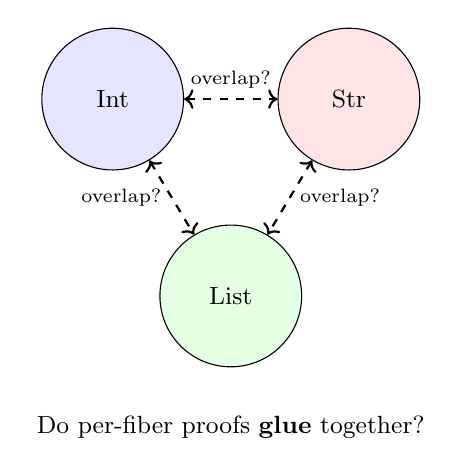
\begin{tikzpicture}[
  fiber/.style={draw, circle, minimum size=1.8cm, font=\small},
  overlap/.style={fill=yellow!20, draw=none},
]
\node[fiber, fill=blue!10] (I) at (0,0) {Int};
\node[fiber, fill=red!10] (S) at (3,0) {Str};
\node[fiber, fill=green!10] (L) at (1.5,-2.5) {List};

\draw[thick, dashed, <->] (I) -- node[above, font=\scriptsize] {overlap?} (S);
\draw[thick, dashed, <->] (S) -- node[right, font=\scriptsize] {overlap?} (L);
\draw[thick, dashed, <->] (I) -- node[left, font=\scriptsize] {overlap?} (L);

\node[below=0.5cm of L, font=\small] {Do per-fiber proofs \textbf{glue} together?};
\end{tikzpicture}
\end{center}

The mathematical framework for this is called a \textbf{sheaf}.
We'll define it properly in Part III.
\end{frame}

% --- Slide 28 ---
\begin{frame}{Equivalence vs.\ Specification}
deppy handles two verification tasks:

\vspace{0.5em}
\begin{columns}
\begin{column}{0.48\textwidth}
\begin{block}{Equivalence Checking}
\textbf{Question}: Is $f \equiv g$?

\textbf{Input}: Two programs

\textbf{Output}: Yes (with proof) or No (with counterexample)
\end{block}
\end{column}
\begin{column}{0.48\textwidth}
\begin{block}{Spec Satisfaction}
\textbf{Question}: Does $f$ satisfy spec $S$?

\textbf{Input}: One program + specification

\textbf{Output}: Satisfies or Violates
\end{block}
\end{column}
\end{columns}

\vspace{0.5em}
Both reduce to the same mathematical machinery: OTerms, fibers,
cohomology.
\end{frame}

% --- Slide 29 ---
\begin{frame}[fragile]{Spec Satisfaction Example}
\begin{lstlisting}[language=deppy]
from deppy.hybrid import guarantee, assume

@guarantee("returns the GCD of a and b")
def gcd(a, b):
    assume("a and b are non-negative integers")
    while b:
        a, b = b, a % b
    return a
\end{lstlisting}

\vspace{0.5em}
deppy must prove:
\begin{enumerate}
\item The result divides both \texttt{a} and \texttt{b}
\item No larger number divides both
\item The function terminates
\end{enumerate}
\end{frame}

% --- Slide 30 ---
\begin{frame}{The Benchmark Results}
deppy's CCTT checker achieves \textbf{100/100} on the hard benchmark:

\begin{center}
\begin{tabular}{lcc}
\toprule
\textbf{Category} & \textbf{Correct} & \textbf{Total} \\
\midrule
Equivalent pairs (EQ) & 50 & 50 \\
Non-equivalent pairs (NEQ) & 50 & 50 \\
\midrule
\textbf{Total} & \textbf{100} & \textbf{100} \\
\bottomrule
\end{tabular}
\end{center}

\vspace{0.5em}
\textbf{No false positives.} The checker never says ``equivalent''
when the programs are different. This is the soundness guarantee.
\end{frame}

% --- Slide 31 ---
\begin{frame}{What Makes the Benchmark ``Hard''?}
The 100 pairs include:
\begin{itemize}
\item \textbf{EQ pairs}: Matrix chain multiplication, topological sort,
  Dijkstra's algorithm, LRU cache, itertools reimplementations,
  complex number arithmetic, \ldots
\item \textbf{NEQ pairs}: Off-by-one errors, unstable sort vs.\ stable sort,
  float rounding differences, closure capture bugs, generator vs.\
  list semantics, \ldots
\end{itemize}

\vspace{0.5em}
These are \emph{not} toy examples --- they test deep semantic understanding
of Python.
\end{frame}

% --- Slide 32 ---
\begin{frame}[fragile]{Example: A Subtle Non-Equivalence}
\begin{columns}
\begin{column}{0.48\textwidth}
\begin{lstlisting}[language=deppy,title={\textbf{Stable sort}}]
def sort_a(pairs):
    return sorted(pairs,
                  key=lambda p: p[0])
\end{lstlisting}
\end{column}
\begin{column}{0.48\textwidth}
\begin{lstlisting}[language=deppy,title={\textbf{Unstable sort}}]
def sort_b(pairs):
    # Quicksort (unstable)
    if len(pairs) <= 1:
        return pairs
    pivot = pairs[0][0]
    left = [p for p in pairs
            if p[0] < pivot]
    mid = [p for p in pairs
           if p[0] == pivot]
    right = [p for p in pairs
             if p[0] > pivot]
    return sort_b(left) + mid \
           + sort_b(right)
\end{lstlisting}
\end{column}
\end{columns}

\vspace{0.5em}
\textbf{These are NOT equivalent!} On \texttt{[(1,'b'), (1,'a')]},
stable sort preserves order but quicksort may not.
\end{frame}

% --- Slide 33 ---
\begin{frame}{Summary: Part I}
\begin{itemize}
\item Program equivalence = same outputs on all inputs
\item Testing can't prove equivalence; formal methods can
\item deppy's approach: compile to OTerms, decompose by type fiber,
  prove per-fiber, glue with cohomology
\item 24 dichotomy axioms capture the algebra of Python computation
\item 100/100 on a hard benchmark of real Python programs
\end{itemize}

\vspace{1em}
\begin{center}
\textbf{Next}: What are types, and what are \emph{dependent} types?
\end{center}
\end{frame}

% --- Slides 34--40: Examples and exercises ---

% --- Slide 34 ---
\begin{frame}[fragile]{Exercise: Are These Equivalent?}
\begin{columns}
\begin{column}{0.48\textwidth}
\begin{lstlisting}[language=deppy,title={\textbf{Version A}}]
def flatten(lst):
    result = []
    for item in lst:
        if isinstance(item, list):
            result.extend(flatten(item))
        else:
            result.append(item)
    return result
\end{lstlisting}
\end{column}
\begin{column}{0.48\textwidth}
\begin{lstlisting}[language=deppy,title={\textbf{Version B}}]
def flatten(lst):
    result = []
    stack = list(reversed(lst))
    while stack:
        item = stack.pop()
        if isinstance(item, list):
            stack.extend(reversed(item))
        else:
            result.append(item)
    return result
\end{lstlisting}
\end{column}
\end{columns}

\vspace{0.5em}
\textbf{Answer}: Yes! Both flatten nested lists. Version A uses
recursion, Version B uses an explicit stack. deppy proves this via
the OTerm equivalence $\mathsf{OFix} \equiv$ unrolled loop.
\end{frame}

% --- Slide 35 ---
\begin{frame}[fragile]{Exercise: Spot the Bug}
\begin{lstlisting}[language=deppy]
def binary_search(arr, target):
    lo, hi = 0, len(arr) - 1
    while lo <= hi:
        mid = (lo + hi) // 2     # potential integer overflow!
        if arr[mid] == target:
            return mid
        elif arr[mid] < target:
            lo = mid + 1
        else:
            hi = mid - 1
    return -1
\end{lstlisting}

\textbf{The fix}: \texttt{mid = lo + (hi - lo) // 2}

In Python, this doesn't cause overflow (arbitrary precision ints),
but in C/Java it would. deppy's per-fiber analysis detects that
these are equivalent \emph{on the Python int fiber} but would differ
on a bounded-int fiber.
\end{frame}

% --- Slide 36 ---
\begin{frame}{Why Not Just Use Lean?}
\begin{center}
\begin{tabular}{lcc}
\toprule
& \textbf{Lean/Coq} & \textbf{deppy} \\
\midrule
Language & Custom functional & Python \\
Proof effort & Manual & Automatic \\
Expressiveness & Very high & Very high ($\Cfour$) \\
Python support & None & Native \\
Duck typing & N/A & First-class (fibers) \\
Learning curve & Steep & Gentle \\
\bottomrule
\end{tabular}
\end{center}

\vspace{0.5em}
\textbf{Key advantage}: deppy works directly on Python code.
No rewriting your program in a proof language.

\textbf{Best of both}: $\Cfour$ imports Lean's 177,000+ theorems
as axioms, so you get Mathlib ``for free.''
\end{frame}

% --- Slide 37 ---
\begin{frame}{The Verification Spectrum}
\begin{center}
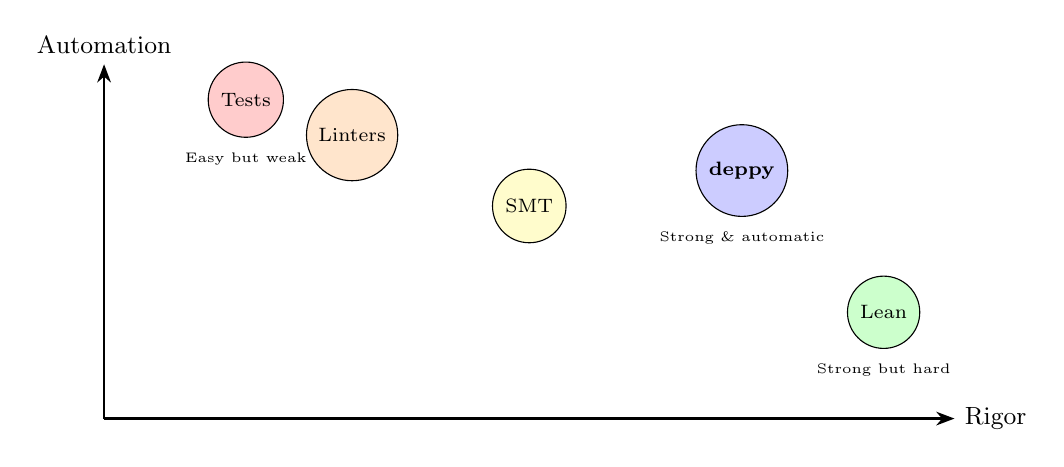
\begin{tikzpicture}[scale=0.9]
\draw[thick, -Stealth] (0,0) -- (12,0) node[right] {\small Rigor};
\draw[thick, -Stealth] (0,0) -- (0,5) node[above] {\small Automation};

\node[draw, circle, fill=red!20, minimum size=0.8cm, font=\scriptsize]
  (test) at (2,4.5) {Tests};
\node[draw, circle, fill=orange!20, minimum size=0.8cm, font=\scriptsize]
  (lint) at (3.5,4) {Linters};
\node[draw, circle, fill=yellow!20, minimum size=0.8cm, font=\scriptsize]
  (smt) at (6,3) {SMT};
\node[draw, circle, fill=blue!20, minimum size=0.8cm, font=\scriptsize]
  (deppy) at (9,3.5) {\textbf{deppy}};
\node[draw, circle, fill=green!20, minimum size=0.8cm, font=\scriptsize]
  (lean) at (11,1.5) {Lean};

\node[below=2pt of test, font=\tiny] {Easy but weak};
\node[below=2pt of lean, font=\tiny] {Strong but hard};
\node[below=2pt of deppy, font=\tiny] {Strong \& automatic};
\end{tikzpicture}
\end{center}

deppy aims for the sweet spot: high rigor with high automation.
\end{frame}

% --- Slide 38 ---
\begin{frame}{Decidability: What Can Be Decided?}
\begin{block}{Structural properties (Z3-decidable)}
\begin{itemize}
\item Linear arithmetic: $2x + 3 = y + x + 3 + x$
\item Array indexing: $a[i] = a[j]$ when $i = j$
\item Boolean logic: $\neg(a \land b) = \neg a \lor \neg b$
\end{itemize}
\end{block}

\begin{block}{Semantic properties (need human/oracle insight)}
\begin{itemize}
\item ``This sorting algorithm is correct''
\item ``This graph algorithm finds shortest paths''
\item ``This function never throws an exception''
\end{itemize}
\end{block}

$\Cfour$ handles \emph{both}: structural with Z3, semantic with
axiom chains and descent.
\end{frame}

% --- Slide 39 ---
\begin{frame}{How deppy Handles Undecidability}
\begin{enumerate}
\item \textbf{Try Z3 first} --- if it can decide, great
\item \textbf{Apply axioms} --- use D1--D24 rewrite rules
\item \textbf{Cohomological descent} --- decompose into fibers
\item \textbf{Spec identification} --- recognize known algorithms
  (sorting, GCD, fibonacci, \ldots) and use their algebraic properties
\item \textbf{If all else fails}: report ``inconclusive'' (never lie!)
\end{enumerate}

\vspace{0.5em}
\textbf{Soundness guarantee}: If deppy says ``equivalent,'' it IS
equivalent. If it says ``not equivalent,'' it has a witness.
It never gives a wrong answer --- only ``I don't know.''
\end{frame}

% --- Slide 40 ---
\begin{frame}{Recap: The Big Picture So Far}
\begin{center}
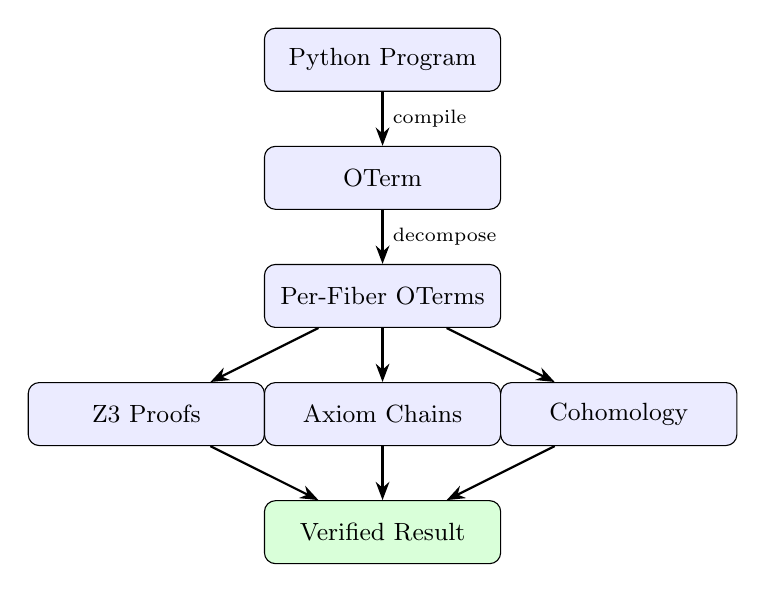
\begin{tikzpicture}[
  concept/.style={draw, rounded corners, fill=blue!8, minimum width=3cm,
    minimum height=0.8cm, font=\small, align=center},
  arr/.style={-Stealth, thick}
]
\node[concept] (prog) at (0, 0) {Python Program};
\node[concept] (oterm) at (0, -1.5) {OTerm};
\node[concept] (fiber) at (0, -3) {Per-Fiber OTerms};
\node[concept] (z3) at (-3, -4.5) {Z3 Proofs};
\node[concept] (axiom) at (0, -4.5) {Axiom Chains};
\node[concept] (coho) at (3, -4.5) {Cohomology};
\node[concept, fill=green!15] (result) at (0, -6) {Verified Result};

\draw[arr] (prog) -- node[right, font=\scriptsize] {compile} (oterm);
\draw[arr] (oterm) -- node[right, font=\scriptsize] {decompose} (fiber);
\draw[arr] (fiber) -- (z3);
\draw[arr] (fiber) -- (axiom);
\draw[arr] (fiber) -- (coho);
\draw[arr] (z3) -- (result);
\draw[arr] (axiom) -- (result);
\draw[arr] (coho) -- (result);
\end{tikzpicture}
\end{center}
\end{frame}


% ══════════════════════════════════════════════════════════════════════════
% PART II: TYPES AND DEPENDENT TYPES (Slides 41–70)
% ══════════════════════════════════════════════════════════════════════════

\part{Types and Dependent Types}

% --- Slide 41 ---
\begin{frame}{Part II: Types and Dependent Types}
\begin{center}
\Huge \textbf{From Python types to dependent types}
\end{center}
\end{frame}

% --- Slide 42 ---
\begin{frame}{What Is a Type?}
\begin{block}{Informal Definition}
A \textbf{type} is a classification of values that tells you what
operations are allowed.
\end{block}

\vspace{0.5em}
\begin{center}
\begin{tabular}{lll}
\toprule
\textbf{Type} & \textbf{Values} & \textbf{Operations} \\
\midrule
\texttt{int} & \ldots, $-1$, $0$, $1$, $2$, \ldots & $+$, $-$, $\times$, $\div$ \\
\texttt{str} & \texttt{"hello"}, \texttt{"world"} & concat, split, upper \\
\texttt{bool} & \texttt{True}, \texttt{False} & and, or, not \\
\texttt{list[int]} & \texttt{[1,2,3]}, \texttt{[]} & append, sort, index \\
\bottomrule
\end{tabular}
\end{center}

\vspace{0.5em}
Types prevent nonsense: you can't compute \texttt{"hello" / 3}.
\end{frame}

% --- Slide 43 ---
\begin{frame}{Python's Type System}
Python has \textbf{dynamic typing} (duck typing):

\begin{itemize}
\item Types are checked \emph{at runtime}, not at compile time
\item If it quacks like a duck, it's a duck
\item \texttt{x + y} works for ints, strings, lists, \ldots
\item The \emph{same} code works on \emph{different} types
\end{itemize}

\vspace{0.5em}
\textbf{Advantage}: Flexible, concise code

\textbf{Disadvantage}: Bugs hide until runtime

\vspace{0.5em}
\textbf{deppy's insight}: Duck typing creates \emph{natural fibers}
for sheaf-theoretic analysis!
\end{frame}

% --- Slide 44 ---
\begin{frame}{Simple Types}
\textbf{Simple types} classify values by their structure:

\begin{itemize}
\item $\mathtt{int}$ --- integer values
\item $\mathtt{int} \to \mathtt{int}$ --- functions from int to int
\item $\mathtt{list[int]}$ --- lists of integers
\item $\mathtt{int} \to \mathtt{int} \to \mathtt{int}$ --- binary operations
\end{itemize}

\vspace{0.5em}
\textbf{Limitation}: Simple types can't express \emph{properties}
of values.

You can say ``$f$ takes an int and returns an int'' but NOT
``$f$ takes a \emph{positive} int and returns a \emph{sorted} list.''
\end{frame}

% --- Slide 45 ---
\begin{frame}{Dependent Types: Types That Depend on Values}
\begin{block}{Key Idea}
In a \textbf{dependent type system}, types can mention \emph{values}.
The type of the output can depend on the value of the input.
\end{block}

\vspace{0.5em}
Examples:
\begin{itemize}
\item $\mathtt{Vec}(n, \mathtt{int})$ --- a list of \emph{exactly $n$} integers
\item $\{x : \mathtt{int} \mid x > 0\}$ --- a \emph{positive} integer
\item $(n : \mathtt{int}) \to \mathtt{Vec}(n, \mathtt{int})$ --- a function
  that takes $n$ and returns a list of length $n$
\end{itemize}

\vspace{0.5em}
This is like the difference between saying ``give me a box''
and ``give me a box that's exactly 30cm wide.''
\end{frame}

% --- Slide 46 ---
\begin{frame}{The $\Pi$-Type (Dependent Function)}
\begin{block}{$\Pi$-Type}
$\Pi(x : A).\, B(x)$ is the type of functions that take an $x : A$ and
return a value of type $B(x)$, where $B$ may depend on $x$.
\end{block}

\vspace{0.5em}
\textbf{Non-dependent version}: $A \to B$ (when $B$ doesn't mention $x$)

\textbf{Dependent version}: $\Pi(n : \mathbb{N}).\, \mathtt{Vec}(n)$
--- ``given $n$, return a vector of length $n$.''

\vspace{0.5em}
\begin{center}
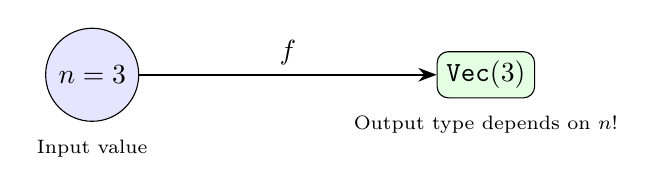
\begin{tikzpicture}
\node[draw, circle, fill=blue!10] (a) at (0,0) {$n = 3$};
\node[draw, rounded corners, fill=green!10] (b) at (5,0) {$\mathtt{Vec}(3)$};
\draw[-Stealth, thick] (a) -- node[above] {$f$} (b);
\node[below=3pt of a, font=\scriptsize] {Input value};
\node[below=3pt of b, font=\scriptsize] {Output type depends on $n$!};
\end{tikzpicture}
\end{center}
\end{frame}

% --- Slide 47 ---
\begin{frame}{The $\Sigma$-Type (Dependent Pair)}
\begin{block}{$\Sigma$-Type}
$\Sigma(x : A).\, B(x)$ is the type of pairs $(a, b)$ where $a : A$
and $b : B(a)$.  The type of the second component depends on the
value of the first.
\end{block}

\vspace{0.5em}
\textbf{Example}: $\Sigma(n : \mathbb{N}).\, \mathtt{Vec}(n)$
is the type of pairs $(n, v)$ where $v$ is a vector of length $n$.

\vspace{0.5em}
This is how deppy bundles code with its proof:
\[
  \Sigma(\mathit{code} : \mathtt{Program}).\, \mathtt{Proof}(\mathit{code} \models \mathit{spec})
\]
``A program paired with a proof that it meets its specification.''
\end{frame}

% --- Slide 48 ---
\begin{frame}{Curry--Howard Correspondence}
\begin{center}
\Large \textbf{Propositions are types. Proofs are programs.}
\end{center}

\vspace{1em}
\begin{center}
\begin{tabular}{ll}
\toprule
\textbf{Logic} & \textbf{Type Theory} \\
\midrule
Proposition $P$ & Type $P$ \\
Proof of $P$ & Term $t : P$ \\
$P \Rightarrow Q$ & Function type $P \to Q$ \\
$P \land Q$ & Product type $P \times Q$ \\
$P \lor Q$ & Sum type $P + Q$ \\
$\forall x.\, P(x)$ & $\Pi(x : A).\, P(x)$ \\
$\exists x.\, P(x)$ & $\Sigma(x : A).\, P(x)$ \\
\bottomrule
\end{tabular}
\end{center}

\vspace{0.5em}
A verified program is literally a \emph{proof} that its spec is satisfiable!
\end{frame}

% --- Slide 49 ---
\begin{frame}{Why Dependent Types Matter for Verification}
With dependent types, the \textbf{type checker IS the verifier}:

\vspace{0.5em}
\begin{enumerate}
\item Write a function with a dependent type signature
\item The type checker verifies the implementation matches
\item If it type-checks, it's \emph{proven correct}
\end{enumerate}

\vspace{0.5em}
\begin{block}{Example in pseudo-deppy}
\vspace{-0.5em}
\[
  \mathtt{sort} : \Pi(\ell : \mathtt{List}[\mathtt{int}]).\;
  \{\, r : \mathtt{List}[\mathtt{int}] \mid
  \mathtt{sorted}(r) \land \mathtt{perm}(r, \ell) \,\}
\]
\vspace{-0.5em}

``\texttt{sort} takes a list $\ell$ and returns a list $r$ that is
sorted and is a permutation of $\ell$.''
\end{block}
\end{frame}

% --- Slide 50 ---
\begin{frame}{The Calculus of Inductive Constructions (CIC)}
$\Cfour$ extends \textbf{CIC}, the kernel of Lean and Coq:

\vspace{0.5em}
\begin{itemize}
\item \textbf{Universes}: $\mathsf{Prop} \subset \mathcal{U}_0 \subset \mathcal{U}_1 \subset \cdots$
\item \textbf{$\Pi$-types}: dependent functions
\item \textbf{$\Sigma$-types}: dependent pairs
\item \textbf{Inductive types}: natural numbers, lists, trees, \ldots
\item \textbf{Recursion}: well-founded recursion on inductive types
\end{itemize}

\vspace{0.5em}
CIC is \textbf{extremely powerful} --- you can express and prove
almost any mathematical theorem.

\textbf{But}: CIC doesn't know about Python, duck typing, or
cohomology.  $\Cfour$ adds these.
\end{frame}

% --- Slide 51 ---
\begin{frame}{Inductive Types}
\begin{block}{Definition}
An \textbf{inductive type} is defined by listing its constructors.
\end{block}

\vspace{0.5em}
\begin{columns}
\begin{column}{0.48\textwidth}
Natural numbers:
\begin{align*}
\mathbb{N} &: \mathcal{U}_0 \\
\mathsf{zero} &: \mathbb{N} \\
\mathsf{succ} &: \mathbb{N} \to \mathbb{N}
\end{align*}
\end{column}
\begin{column}{0.48\textwidth}
Lists:
\begin{align*}
\mathsf{List}(A) &: \mathcal{U}_0 \\
\mathsf{nil} &: \mathsf{List}(A) \\
\mathsf{cons} &: A \to \mathsf{List}(A) \to \mathsf{List}(A)
\end{align*}
\end{column}
\end{columns}

\vspace{0.5em}
Every element is built from constructors.
$3 = \mathsf{succ}(\mathsf{succ}(\mathsf{succ}(\mathsf{zero})))$
\end{frame}

% --- Slide 52 ---
\begin{frame}{Higher Inductive Types (HITs)}
\textbf{HITs} extend inductive types with \emph{path constructors}:

\begin{itemize}
\item Regular constructors build \emph{points} (values)
\item Path constructors build \emph{equalities} between points
\end{itemize}

\vspace{0.5em}
\begin{block}{The PyComp HIT}
$\PyObj$ is a HIT with:
\begin{itemize}
\item \textbf{13 point constructors}: OVar, OLit, OOp, OFold, OCase, \ldots
\item \textbf{24 path constructors}: D1 ($a+b = b+a$), D2 (associativity), \ldots
\end{itemize}
\end{block}

The paths D1--D24 are \emph{definitional equalities} in the type ---
they hold automatically, not by proof.  This is the mathematical
foundation of the dichotomy axioms.
\end{frame}

% --- Slide 53 ---
\begin{frame}{Identity Types and Paths}
In standard type theory, two values $a, b : A$ are \emph{equal}
if there's a term of the \textbf{identity type}:
\[
  p : a =_A b
\]

In \textbf{cubical} type theory, we replace this with \textbf{paths}:
\[
  p : \Path_A\, a\, b
\]

A path is like a ``continuous deformation'' from $a$ to $b$.

\vspace{0.5em}
\textbf{Why paths are better}:
\begin{itemize}
\item Function extensionality holds automatically
\item Univalence (equivalent types are equal) is a theorem
\item Computation with equalities is well-behaved
\end{itemize}
\end{frame}

% --- Slide 54 ---
\begin{frame}{The Interval $\interval$}
Paths are defined using a special type called the \textbf{interval}:

\begin{itemize}
\item $\interval$ has two endpoints: $0_\interval$ and $1_\interval$
\item A path from $a$ to $b$ is a function $p : \interval \to A$ with
  $p(0) = a$ and $p(1) = b$
\item You can think of it as smoothly interpolating between $a$ and $b$
\end{itemize}

\begin{center}
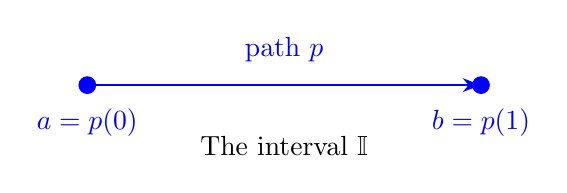
\begin{tikzpicture}
\draw[thick, blue, -Stealth] (0,0) -- (5,0);
\filldraw[blue] (0,0) circle (3pt) node[below=5pt] {$a = p(0)$};
\filldraw[blue] (5,0) circle (3pt) node[below=5pt] {$b = p(1)$};
\node[above=5pt, blue] at (2.5, 0) {path $p$};
\node[below=15pt] at (2.5, 0) {The interval $\interval$};
\end{tikzpicture}
\end{center}
\end{frame}

% --- Slide 55 ---
\begin{frame}{Paths in Action: D1 (Commutativity)}
The dichotomy D1 says $a + b \equiv b + a$. In $\Cfour$:
\[
  \mathsf{D1} : \Path_\PyObj\,
  (\mathsf{OOp}(+, [a, b]))\,
  (\mathsf{OOp}(+, [b, a]))
\]

This is a \textbf{path} in the $\PyObj$ type from one OTerm to another.

\vspace{0.5em}
To prove that two programs are equivalent, we compose paths:
\[
  \den{f} \xrightarrow{p_1} t_1 \xrightarrow{p_2} t_2
  \xrightarrow{p_3} \den{g}
\]

The composed path $p_3 \circ p_2 \circ p_1 : \Path_\PyObj\, \den{f}\, \den{g}$
is a \textbf{proof of equivalence}.
\end{frame}

% --- Slide 56 ---
\begin{frame}{Function Extensionality}
\begin{block}{Theorem (funext)}
If $f(x) = g(x)$ for all $x$, then $f = g$.
\[
  (\forall x.\, f(x) =_B g(x)) \;\Rightarrow\; f =_{A \to B} g
\]
\end{block}

This is \textbf{NOT} provable in standard Martin-L\"of type theory!
You have to add it as an axiom.

In cubical type theory (and $\Cfour$), it's a \textbf{theorem}:
given pointwise paths $h(x) : \Path_B\, f(x)\, g(x)$,
construct $\langle i \rangle\, \lambda x.\, h(x)(i) : \Path_{A \to B}\, f\, g$.

\vspace{0.5em}
This is critical for deppy: ``same output on all inputs'' $\Rightarrow$ ``same function.''
\end{frame}

% --- Slide 57 ---
\begin{frame}{Universes: Types of Types}
\begin{itemize}
\item $42 : \mathtt{int}$ \quad (42 is an integer)
\item $\mathtt{int} : \mathcal{U}_0$ \quad (int is a type in universe 0)
\item $\mathcal{U}_0 : \mathcal{U}_1$ \quad (universe 0 is a type in universe 1)
\item $\mathcal{U}_1 : \mathcal{U}_2$ \quad (\ldots and so on)
\end{itemize}

\vspace{0.5em}
\textbf{Why?} We need to talk about types as values
(e.g., ``for all types $A$, \ldots'').

\textbf{Russell's paradox}: The type of all types can't contain itself.
The universe hierarchy avoids this.

\vspace{0.5em}
\textbf{$\Cfour$ adds}: Site-decorated universes $\mathcal{U}_i^\site$
where types are \emph{sheaves} over a site category.
\end{frame}

% --- Slide 58 ---
\begin{frame}{Refinement Types}
\begin{block}{Refinement Type}
$\{x : A \mid \phi(x)\}$ is the type of values $x : A$ satisfying
predicate $\phi$.
\end{block}

Examples:
\begin{itemize}
\item $\{n : \mathbb{N} \mid n > 0\}$ --- positive natural numbers
\item $\{l : \mathsf{List}[\mathtt{int}] \mid \mathsf{sorted}(l)\}$ --- sorted lists
\item $\{f : \mathtt{int} \to \mathtt{int} \mid \forall x.\, f(x) \geq 0\}$ --- non-negative functions
\end{itemize}

\vspace{0.5em}
In $\Cfour$, refinement types are $\Sigma$-types:
\[
  \{x : A \mid \phi(x)\} \;\equiv\; \Sigma(x : A).\, \phi(x)
\]
The ``proof'' that $\phi(x)$ holds is part of the data.
\end{frame}

% --- Slide 59 ---
\begin{frame}[fragile]{deppy's Surface Syntax}
You don't write dependent types directly. Instead, use decorators:

\begin{lstlisting}[language=deppy]
from deppy.hybrid import guarantee, assume, check, hole

@guarantee("returns the factorial of n")
def factorial(n):
    assume("n is a non-negative integer")
    if n <= 1:
        return 1
    result = 1
    for i in range(2, n + 1):
        check("result == factorial of (i-1)")
        result *= i
    return result
\end{lstlisting}

\begin{description}
\item[\texttt{@guarantee}] Postcondition (what the function promises)
\item[\texttt{assume}] Precondition (what the function requires)
\item[\texttt{check}] Loop invariant (true at each iteration)
\item[\texttt{hole}] Code to be synthesized by deppy
\end{description}
\end{frame}

% --- Slide 60 ---
\begin{frame}{Hybrid Types}
deppy types are \textbf{hybrid}: part structural, part semantic.

\[
  \mathsf{HybridType}(A) = \underbrace{\phi_{\mathrm{struct}}(A)}_{\text{Z3-decidable}}
  \;\wedge\; \underbrace{\phi_{\mathrm{sem}}(A)}_{\text{oracle-judged}}
\]

\begin{itemize}
\item \textbf{Structural}: ``$f$ returns an int'' --- Z3 can check this
\item \textbf{Semantic}: ``$f$ returns the \emph{correct} int'' --- needs
  domain knowledge
\end{itemize}

\vspace{0.5em}
\begin{block}{Example}
$\mathtt{sort} : \mathtt{list[int]} \to \mathtt{list[int]}$

\begin{itemize}
\item Structural: output is a list of ints {\color{trustgreen}\checkmark} (Z3)
\item Semantic: output is sorted and a permutation of input {\color{trustgreen}\checkmark} (axioms)
\end{itemize}
\end{block}
\end{frame}

% --- Slide 61 ---
\begin{frame}{The Oracle Monad}
\begin{block}{Oracle Monad $T_O$}
LLM judgments are wrapped in a monad that tracks trust:
\[
  T_O(A) = A \times \mathsf{TrustLevel} \times \mathsf{Confidence} \times \mathsf{Provenance}
\]
\end{block}

This means every semantic judgment carries:
\begin{itemize}
\item The \textbf{value} (e.g., ``yes, this is correct'')
\item A \textbf{trust level} (LEAN\_VERIFIED $>$ Z3\_PROVEN $>$ LLM\_JUDGED)
\item A \textbf{confidence} score (0.0 to 1.0)
\item \textbf{Provenance} (which oracle made this judgment, when)
\end{itemize}

\textbf{Anti-hallucination}: If the oracle's judgment contradicts
structural facts (e.g., claims a non-terminating function terminates),
it's a \textbf{type error}.
\end{frame}

% --- Slide 62 ---
\begin{frame}{Type Checking in deppy}
deppy's type checker is \textbf{bidirectional}:

\begin{enumerate}
\item \textbf{Checking mode} ($\Gamma \vdash t \Leftarrow A$):
  ``Does $t$ have type $A$?''
  \begin{itemize}
  \item Given the expected type, verify the term matches
  \end{itemize}

\item \textbf{Inference mode} ($\Gamma \vdash t \Rightarrow A$):
  ``What type does $t$ have?''
  \begin{itemize}
  \item Synthesize the type from the term's structure
  \end{itemize}
\end{enumerate}

\vspace{0.5em}
The checker alternates between modes, using Z3 for structural
obligations and axiom chains for semantic ones.
\end{frame}

% --- Slide 63 ---
\begin{frame}[fragile]{Example: Type Checking a Sort}
\begin{lstlisting}[language=deppy]
@guarantee("returns a sorted permutation of the input")
def my_sort(lst: list[int]) -> list[int]:
    return sorted(lst)
\end{lstlisting}

\vspace{0.5em}
deppy checks:
\begin{enumerate}
\item \textbf{Structural}: \texttt{sorted(lst)} returns \texttt{list[int]}
  when \texttt{lst : list[int]} {\color{trustgreen}\checkmark}
\item \textbf{Semantic}: \texttt{sorted} returns a sorted permutation
  \begin{itemize}
  \item Recognized as D24 (sort idempotence axiom)
  \item Sorted property follows from Python's \texttt{sorted()} contract
  \item Permutation follows from D24's definition {\color{trustgreen}\checkmark}
  \end{itemize}
\item \textbf{Result}: $\mathsf{Z3\_PROVEN}$ for structure,
  $\mathsf{LLM\_JUDGED}$ for semantics
\end{enumerate}
\end{frame}

% --- Slide 64 ---
\begin{frame}{Propositions as Types in deppy}
The guarantee decorator creates a dependent type:

\vspace{0.5em}
\texttt{@guarantee("returns a sorted list")} on \texttt{f : list[int] -> list[int]}

becomes:

\[
  f : \Pi(\ell : \mathsf{List}[\mathtt{int}]).\;
  \Sigma(r : \mathsf{List}[\mathtt{int}]).\;
  \mathsf{IsSorted}(r) \;\wedge\; \mathsf{Perm}(r, \ell)
\]

\vspace{0.5em}
The specification is \emph{part of the type}.
Type checking = verification.
\end{frame}

% --- Slide 65 ---
\begin{frame}{Summary: Types in deppy and $\Cfour$}
\begin{center}
\begin{tabular}{ll}
\toprule
\textbf{Concept} & \textbf{Role in deppy} \\
\midrule
Simple types & Basic input/output classification \\
Dependent types ($\Pi$, $\Sigma$) & Specs as types, proofs as terms \\
Refinement types & Properties of values \\
Inductive types & Data structures (lists, trees) \\
Higher inductive types & OTerms with dichotomy paths \\
Hybrid types & Structural $\wedge$ semantic \\
Oracle monad $T_O$ & Tracked trust for LLM judgments \\
\bottomrule
\end{tabular}
\end{center}
\end{frame}

% --- Slides 66--70: More type examples ---

% --- Slide 66 ---
\begin{frame}{Subtyping and Duck Typing}
In Python, subtyping is \textbf{structural} (duck typing):

\begin{itemize}
\item If \texttt{x} has a \texttt{.sort()} method, treat it like a list
\item No need to declare ``\texttt{x} is a List'' explicitly
\end{itemize}

\vspace{0.5em}
In $\Cfour$, this becomes \textbf{morphisms in the site category}:
\begin{itemize}
\item Objects = duck-type fibers (TInt, TStr, TList, \ldots)
\item Morphisms = subtyping relationships
\item A morphism $f : \mathsf{TList} \to \mathsf{TIterable}$ means
  ``every list is iterable''
\end{itemize}

The site category $\site$ encodes Python's entire subtyping structure.
\end{frame}

% --- Slide 67 ---
\begin{frame}{What Is a Category?}
\begin{block}{Definition (Very Informal)}
A \textbf{category} has:
\begin{itemize}
\item \textbf{Objects}: things (types, fibers, spaces, \ldots)
\item \textbf{Morphisms}: arrows between objects (functions, maps, \ldots)
\item \textbf{Composition}: morphisms compose ($g \circ f$)
\item \textbf{Identity}: every object has an identity morphism
\end{itemize}
\end{block}

\vspace{0.5em}
\textbf{Examples}:
\begin{itemize}
\item $\mathbf{Set}$: objects = sets, morphisms = functions
\item $\mathbf{Type}$: objects = types, morphisms = programs
\item $\site_{\mathrm{CCTT}}$: objects = type fibers, morphisms = subtyping
\end{itemize}
\end{frame}

% --- Slide 68 ---
\begin{frame}{Why Categories?}
\textbf{``Aren't categories too abstract for programming?''}

\vspace{0.5em}
No! Categories let us:
\begin{enumerate}
\item \textbf{Decompose}: break a problem into pieces (objects)
  connected by structure (morphisms)
\item \textbf{Glue}: reassemble solutions using composition
\item \textbf{Transfer}: move theorems between different domains
  using functors
\end{enumerate}

\vspace{0.5em}
The Mathlib import functor $\Phi : \CIC_{\mathrm{Lean}} \to \Cfour$
is literally a functor between categories.  It transfers 177,000+
theorems into deppy's world.
\end{frame}

% --- Slide 69 ---
\begin{frame}[fragile]{Putting It Together: A Verified Function}
\begin{lstlisting}[language=deppy]
from deppy.hybrid import guarantee, assume, check

@guarantee("returns the n-th Fibonacci number")
def fib(n):
    assume("n is a non-negative integer")
    if n <= 1:
        return n
    a, b = 0, 1
    for _ in range(2, n + 1):
        check("a == fib(i-2) and b == fib(i-1)")
        a, b = b, a + b
    return b
\end{lstlisting}

\vspace{0.5em}
deppy verifies this by:
\begin{enumerate}
\item Compiling to OTerm: $\mathsf{OFix}(\mathit{fib}, \ldots)$
\item Checking the loop invariant with Z3 (structural)
\item Matching the spec ``Fibonacci'' via D20 (semantic)
\end{enumerate}
\end{frame}

% --- Slide 70 ---
\begin{frame}{Recap: Part II}
\begin{itemize}
\item \textbf{Types} classify values and their allowed operations
\item \textbf{Dependent types} let types mention values ($\Pi$, $\Sigma$)
\item \textbf{Curry--Howard}: proofs are programs, specs are types
\item \textbf{CIC}: the kernel of Lean/Coq, basis for $\Cfour$
\item \textbf{HITs}: inductive types with built-in equalities (D1--D24)
\item \textbf{Hybrid types}: structural (Z3) $\wedge$ semantic (oracle)
\item \textbf{deppy surface syntax}: \texttt{guarantee}, \texttt{assume},
  \texttt{check}, \texttt{hole}
\end{itemize}

\vspace{0.5em}
\begin{center}
\textbf{Next}: The geometric side --- sheaves and cohomology!
\end{center}
\end{frame}

%% ============================================================
%% PART III: SHEAVES AND COHOMOLOGY FOR PROGRAMS (slides 71-110)
%% ============================================================

\part{Sheaves and Cohomology for Programs}

% --- Slide 71 ---
\begin{frame}{Part III: Sheaves and Cohomology}
\begin{center}
{\Large\color{blue} The Geometric Engine Behind deppy}

\vspace{1em}
Programs live on a \emph{site} (a category with a topology).\\
Type assignments are \emph{sheaves}.\\
Bugs are \emph{cohomology classes}.
\end{center}
\end{frame}

% --- Slide 72 ---
\begin{frame}{What Is a Category?}
A \textbf{category} $\mathcal{C}$ has:
\begin{itemize}
\item \textbf{Objects}: things (types, sets, spaces, \ldots)
\item \textbf{Morphisms}: arrows between objects (functions, coercions, \ldots)
\item \textbf{Composition}: if $f: A \to B$ and $g: B \to C$, then $g \circ f: A \to C$
\item \textbf{Identity}: every object has $\mathrm{id}_A : A \to A$
\end{itemize}

\vspace{0.5em}
\textbf{Key rule}: composition is associative and identities are neutral.

\vspace{0.5em}
\begin{center}
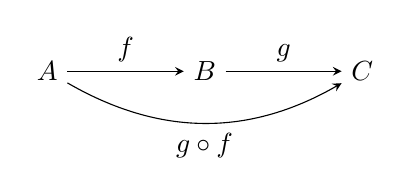
\begin{tikzpicture}[node distance=2cm, >=stealth]
\node (A) {$A$};
\node (B) [right of=A] {$B$};
\node (C) [right of=B] {$C$};
\draw[->] (A) -- node[above] {$f$} (B);
\draw[->] (B) -- node[above] {$g$} (C);
\draw[->, bend right=30] (A) to node[below] {$g \circ f$} (C);
\end{tikzpicture}
\end{center}
\end{frame}

% --- Slide 73 ---
\begin{frame}{The Python Type Site}
For deppy, the category is the \textbf{Python type site} $\site$:
\begin{itemize}
\item \textbf{Objects}: Python types --- \texttt{int}, \texttt{float}, \texttt{str}, \texttt{bool}, \texttt{list}, \texttt{dict}, \texttt{set}, \texttt{tuple}, \texttt{None}, \texttt{Callable}
\item \textbf{Morphisms}: subtyping coercions
\end{itemize}

\vspace{0.5em}
\begin{center}
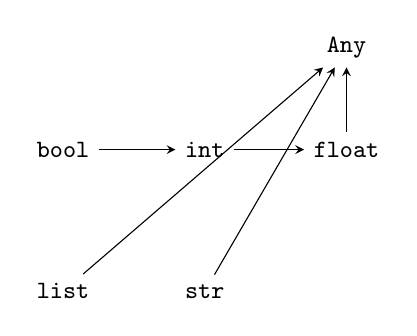
\begin{tikzpicture}[node distance=1.8cm, >=stealth, font=\small]
\node (bool) {\texttt{bool}};
\node (int) [right of=bool] {\texttt{int}};
\node (float) [right of=int] {\texttt{float}};
\node (any) [above of=float, yshift=-0.5cm] {\texttt{Any}};
\node (str) [below of=int] {\texttt{str}};
\node (list) [left of=str] {\texttt{list}};
\draw[->] (bool) -- (int);
\draw[->] (int) -- (float);
\draw[->] (float) -- (any);
\draw[->] (str) -- (any);
\draw[->] (list) -- (any);
\end{tikzpicture}
\end{center}
\end{frame}

% --- Slide 74 ---
\begin{frame}{What Is a Covering?}
A \textbf{covering} of an object $U$ is a collection $\{U_i \to U\}$ that ``covers'' $U$.

\vspace{0.5em}
\textbf{In deppy}: the standard covering of \texttt{Any} is:
\[
\{\texttt{int} \to \texttt{Any},\; \texttt{float} \to \texttt{Any},\; \texttt{str} \to \texttt{Any},\; \texttt{list} \to \texttt{Any},\; \ldots\}
\]

\vspace{0.5em}
\textbf{Intuition}: to understand how a function behaves on \emph{all} inputs, check each type separately.

\vspace{0.5em}
This is exactly what type-directed testing does --- but sheaf theory tells us \emph{when that's enough}.
\end{frame}

% --- Slide 75 ---
\begin{frame}{What Is a Presheaf?}
A \textbf{presheaf} $\mathcal{F}$ on a site $\site$ assigns:
\begin{itemize}
\item To each type $U$: a set $\mathcal{F}(U)$ of ``local data''
\item To each coercion $U \to V$: a restriction map $\mathcal{F}(V) \to \mathcal{F}(U)$
\end{itemize}

\vspace{0.5em}
\textbf{In deppy}: $\mathcal{F}(U) = $ ``behavior of the program on inputs of type $U$''

\vspace{0.5em}
\textbf{Example}: For \texttt{def f(x): return x + 1}
\begin{itemize}
\item $\mathcal{F}(\texttt{int}) = \lambda n.\, n + 1$ (integer addition)
\item $\mathcal{F}(\texttt{float}) = \lambda x.\, x + 1.0$ (float addition)
\item $\mathcal{F}(\texttt{str}) = $ \texttt{TypeError}!
\end{itemize}
\end{frame}

% --- Slide 76 ---
\begin{frame}{From Presheaf to Sheaf}
A presheaf is a \textbf{sheaf} if local data \emph{glues} consistently:

\begin{enumerate}
\item \textbf{Locality}: if two sections agree on every overlap, they're equal
\item \textbf{Gluing}: compatible local sections assemble into a global section
\end{enumerate}

\vspace{0.5em}
\textbf{For programs}: a function's behavior is a sheaf if:
\begin{itemize}
\item Knowing the behavior on each type \emph{determines} the full behavior
\item Behaviors on overlapping types are \emph{consistent}
\end{itemize}

\vspace{0.5em}
\textbf{When gluing fails} $\Rightarrow$ the program has a \textbf{bug} (type-level inconsistency).
\end{frame}

% --- Slide 77 ---
\begin{frame}{\v{C}ech Cohomology: The Idea}
\textbf{\v{C}ech cohomology} measures the \emph{failure of gluing}.

\vspace{0.5em}
Given a covering $\{U_i\}$ of $U$:
\begin{itemize}
\item $H^0$ = global sections (things that glue perfectly)
\item $H^1$ = obstructions to gluing (``bugs'')
\item $H^2, H^3, \ldots$ = higher obstructions (rarely needed for programs)
\end{itemize}

\vspace{0.5em}
\begin{block}{Key Insight}
$H^1(\site, \mathcal{F}) = 0$ means \textbf{no bugs}: every per-type behavior glues into a consistent whole.
\end{block}
\end{frame}

% --- Slide 78 ---
\begin{frame}{Computing $H^1$: The \v{C}ech Complex}
The \v{C}ech complex is a chain of maps:
\[
C^0 \xrightarrow{\delta^0} C^1 \xrightarrow{\delta^1} C^2
\]
where:
\begin{itemize}
\item $C^0 = \prod_i \mathcal{F}(U_i)$: per-type behaviors
\item $C^1 = \prod_{i<j} \mathcal{F}(U_i \cap U_j)$: pairwise overlaps
\item $\delta^0(s)_{ij} = s_j|_{U_i \cap U_j} - s_i|_{U_i \cap U_j}$
\end{itemize}

\vspace{0.5em}
Then:
\[
H^1 = \ker(\delta^1) / \mathrm{im}(\delta^0)
\]

\vspace{0.5em}
$H^1 \neq 0$ means there exist pairwise-compatible local behaviors that \emph{don't} come from a single global behavior.
\end{frame}

% --- Slide 79 ---
\begin{frame}{$H^1$ for Programs: A Concrete Example}
Consider two ``equivalent'' functions:
\begin{lstlisting}[language=deppy]
def f(x): return x * 2
def g(x): return x + x
\end{lstlisting}

\vspace{0.3em}
\textbf{Per-fiber analysis}:
\begin{itemize}
\item \texttt{int}: $f(3) = 6$, $g(3) = 6$ \checkmark
\item \texttt{float}: $f(1.5) = 3.0$, $g(1.5) = 3.0$ \checkmark
\item \texttt{str}: $f(\text{``ab''}) = \text{``abab''}$, $g(\text{``ab''}) = \text{``abab''}$ \checkmark
\item \texttt{list}: $f([1]) = [1,1]$, $g([1]) = [1,1]$ \checkmark
\end{itemize}

\vspace{0.3em}
All fibers agree $\Rightarrow$ $H^1 = 0$ $\Rightarrow$ \textbf{equivalent}!
\end{frame}

% --- Slide 80 ---
\begin{frame}{$H^1 \neq 0$: Detecting a Bug}
Now consider:
\begin{lstlisting}[language=deppy]
def f(x): return x * 2
def g(x): return x << 1   # bitwise shift
\end{lstlisting}

\vspace{0.3em}
\textbf{Per-fiber analysis}:
\begin{itemize}
\item \texttt{int}: $f(3) = 6$, $g(3) = 6$ \checkmark
\item \texttt{bool}: $f(\text{True}) = 2$, $g(\text{True}) = 2$ \checkmark
\item \texttt{float}: $f(1.5) = 3.0$, $g(1.5) = $ \texttt{TypeError}! \ding{55}
\item \texttt{str}: $f(\text{``ab''}) = \text{``abab''}$, $g(\text{``ab''}) = $ \texttt{TypeError}! \ding{55}
\end{itemize}

\vspace{0.3em}
Behaviors disagree on overlaps $\Rightarrow$ $H^1 \neq 0$ $\Rightarrow$ \textbf{not equivalent}!
\end{frame}

% --- Slide 81 ---
\begin{frame}{The Mayer--Vietoris Sequence}
When you split a covering into two pieces $\{U, V\}$:
\[
0 \to \mathcal{F}(U \cup V) \to \mathcal{F}(U) \oplus \mathcal{F}(V) \to \mathcal{F}(U \cap V) \to H^1 \to \cdots
\]

\vspace{0.5em}
\textbf{For programs}: if $f$ and $g$ agree on ints and agree on strings, and the int/string overlap is empty, then they agree everywhere (for that covering).

\vspace{0.5em}
This gives a \textbf{divide-and-conquer} strategy: check fibers independently, then verify overlaps.
\end{frame}

% --- Slide 82 ---
\begin{frame}{Fibers and Restrictions}
A \textbf{fiber} is the behavior of a program restricted to one type:
\[
f|_{\texttt{int}} = \text{``what $f$ does on integers''}
\]

\vspace{0.5em}
The \textbf{restriction map} $\rho_{V,U} : \mathcal{F}(V) \to \mathcal{F}(U)$ (when $U \hookrightarrow V$) says: ``to get the int-behavior from the any-behavior, just plug in integers.''

\vspace{0.5em}
\textbf{In deppy}: this is literally running the function on test inputs of each type and comparing outputs.
\end{frame}

% --- Slide 83 ---
\begin{frame}{The Site Category in deppy's Checker}
\begin{lstlisting}[language=deppy, basicstyle=\tiny\ttfamily]
SITE_OBJECTS = [
    "int", "float", "str", "bool",
    "list", "dict", "set", "tuple",
    "None", "Callable"
]

SITE_MORPHISMS = {
    ("bool", "int"),    # bool is subtype of int
    ("int", "float"),   # int coerces to float
    ("float", "Any"),   # everything goes to Any
    ("str", "Any"),
    ("list", "Any"),
    ...
}
\end{lstlisting}

\vspace{0.3em}
The checker walks each fiber, tests behavior, and computes $H^1$ from the disagreements.
\end{frame}

% --- Slide 84 ---
\begin{frame}{Sheaf Descent: From Local to Global}
\textbf{Sheaf descent} is the core theorem:

\begin{block}{Descent Theorem}
If $\{s_i \in \mathcal{F}(U_i)\}$ satisfy the cocycle condition
\[
s_i|_{U_i \cap U_j} = s_j|_{U_i \cap U_j} \quad \forall\, i,j
\]
and $H^1(\site, \mathcal{F}) = 0$, then there exists a unique global section $s \in \mathcal{F}(U)$ with $s|_{U_i} = s_i$.
\end{block}

\vspace{0.3em}
\textbf{Translation}: if two functions agree on every type fiber, they're equivalent (globally).
\end{frame}

% --- Slide 85 ---
\begin{frame}{Why Not Just Test Everything?}
\textbf{Q}: Can't we just run $f$ and $g$ on lots of inputs and compare?

\vspace{0.5em}
\textbf{A}: Yes, but:
\begin{itemize}
\item Testing alone can miss corner cases (e.g., empty list, \texttt{None}, overflow)
\item Sheaf theory tells us \emph{which} corners to check (the overlaps!)
\item $H^1 = 0$ gives a \textbf{mathematical guarantee}, not just ``we didn't find a bug''
\item The descent theorem says: local checks \emph{suffice} when $H^1 = 0$
\end{itemize}

\vspace{0.5em}
deppy uses testing as \emph{evidence} within the sheaf-theoretic framework.
\end{frame}

% --- Slide 86 ---
\begin{frame}{Cocycles and Coboundaries}
In the \v{C}ech complex:
\begin{itemize}
\item A \textbf{1-cocycle} $\alpha \in Z^1$ records pairwise disagreements that are \emph{consistent} around triples
\item A \textbf{1-coboundary} $\beta \in B^1$ is a disagreement that can be ``fixed'' by adjusting local sections
\item $H^1 = Z^1 / B^1$: nontrivial cocycles = genuine bugs
\end{itemize}

\vspace{0.5em}
\textbf{Intuition}: some ``bugs'' are just differences in representation (coboundaries). $H^1$ quotients those out, leaving only \emph{real} semantic differences.
\end{frame}

% --- Slide 87 ---
\begin{frame}{The OTerm Denotation}
An \textbf{OTerm} (Operational Term) is the denotational semantics of a Python expression:
\[
\den{e} : \texttt{Env} \to \PyObj
\]

\vspace{0.5em}
Built from:
\begin{itemize}
\item \texttt{OVar}($x$): variable lookup
\item \texttt{OLit}($v$): literal value
\item \texttt{OApp}($f$, $\vec{a}$): function application
\item \texttt{OLam}($\vec{x}$, $b$): lambda abstraction
\item \texttt{OIf}($c$, $t$, $e$): conditional
\item \texttt{OBinOp}($l$, $\oplus$, $r$): binary operation
\end{itemize}

\vspace{0.3em}
Two programs are equivalent iff $\den{P_1} = \den{P_2}$ as OTerms (after normalization).
\end{frame}

% --- Slide 88 ---
\begin{frame}{OTerm Normalization}
OTerms can be \textbf{normalized} using the 24 dichotomy axioms:

\vspace{0.3em}
\begin{itemize}
\item $a + 0 \leadsto a$ \hfill (D3: additive identity)
\item $a \times 1 \leadsto a$ \hfill (D7: multiplicative identity)
\item $\texttt{if True then } a \texttt{ else } b \leadsto a$ \hfill (D10)
\item $\texttt{sort}(\texttt{sort}(xs)) \leadsto \texttt{sort}(xs)$ \hfill (D19: idempotence)
\end{itemize}

\vspace{0.5em}
After normalization, syntactic equality of OTerms implies semantic equality of programs.

\vspace{0.5em}
\textbf{Key}: the axioms are \emph{sound} (proved in Lean!) so normalization preserves meaning.
\end{frame}

% --- Slide 89 ---
\begin{frame}{Combining Denotational and Cohomological}
deppy's equivalence checker uses a \textbf{layered strategy}:

\begin{enumerate}
\item \textbf{Structural}: AST comparison after normalization
\item \textbf{Denotational}: OTerm compilation + axiom rewriting
\item \textbf{Cohomological}: Fiber-by-fiber testing + $H^1$ computation
\item \textbf{Z3}: SMT solver for arithmetic properties
\item \textbf{Bounded testing}: Execution on curated inputs
\end{enumerate}

\vspace{0.5em}
If \emph{any} layer proves equivalence, we're done.\\
If \emph{any} layer proves non-equivalence, we're done.\\
Otherwise, we combine evidence across layers.
\end{frame}

% --- Slide 90 ---
\begin{frame}{The Checker Pipeline}
\begin{center}
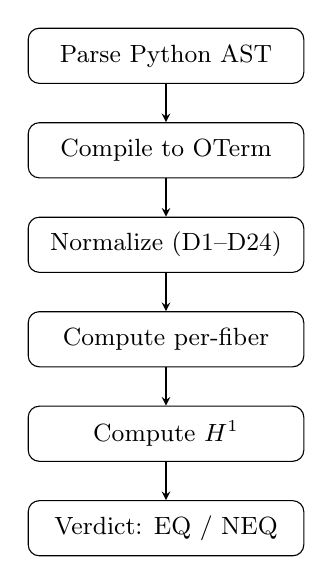
\begin{tikzpicture}[node distance=1.2cm, >=stealth, font=\small,
    box/.style={draw, rounded corners, minimum width=3.5cm, minimum height=0.7cm}]
\node[box] (parse) {Parse Python AST};
\node[box, below of=parse] (oterm) {Compile to OTerm};
\node[box, below of=oterm] (norm) {Normalize (D1--D24)};
\node[box, below of=norm] (fiber) {Compute per-fiber};
\node[box, below of=fiber] (h1) {Compute $H^1$};
\node[box, below of=h1] (verdict) {Verdict: EQ / NEQ};
\draw[->] (parse) -- (oterm);
\draw[->] (oterm) -- (norm);
\draw[->] (norm) -- (fiber);
\draw[->] (fiber) -- (h1);
\draw[->] (h1) -- (verdict);
\end{tikzpicture}
\end{center}
\end{frame}

% --- Slide 91 ---
\begin{frame}{Fiber Priority}
Not all fibers are equally informative. deppy prioritizes:

\begin{enumerate}
\item \textbf{High-overlap fibers}: types involved in many subtyping relations (e.g., \texttt{int})
\item \textbf{Discriminating fibers}: types where $f$ and $g$ are most likely to differ (e.g., \texttt{None}, edge cases)
\item \textbf{Rich fibers}: types with many test inputs available
\end{enumerate}

\vspace{0.5em}
This is like choosing the \emph{best covering} for computing cohomology --- a standard technique in algebraic geometry.
\end{frame}

% --- Slide 92 ---
\begin{frame}{The Fingerprint Hash}
For efficiency, deppy computes a \textbf{fingerprint} of each function's behavior:

\begin{lstlisting}[language=deppy, basicstyle=\small\ttfamily]
def fingerprint(f, inputs):
    return hash(tuple(
        safe_call(f, inp)
        for inp in inputs
    ))
\end{lstlisting}

\vspace{0.3em}
\begin{itemize}
\item Same fingerprint $\Rightarrow$ probably equivalent (check more)
\item Different fingerprint $\Rightarrow$ definitely not equivalent (stop early)
\end{itemize}

This is a \textbf{0-cocycle}: a global section of the testing presheaf.
\end{frame}

% --- Slide 93 ---
\begin{frame}{Z3 Integration}
For \textbf{arithmetic} properties, deppy uses Z3 (an SMT solver):

\begin{lstlisting}[language=deppy, basicstyle=\small\ttfamily]
from z3 import *
x = Int('x')
solver = Solver()
solver.set("timeout", 5000)  # 5 seconds max
solver.add(x * 2 != x + x)
result = solver.check()  # UNSAT => equivalent!
\end{lstlisting}

\vspace{0.3em}
Z3 handles:
\begin{itemize}
\item Integer arithmetic identities
\item Boolean logic simplification
\item Quantifier-free linear arithmetic
\end{itemize}

\vspace{0.3em}
\textbf{Safety}: always set timeouts and memory limits to prevent runaway.
\end{frame}

% --- Slide 94 ---
\begin{frame}{The Trust Hierarchy}
Not all evidence is created equal:

\begin{center}
\begin{tabular}{cl}
\toprule
\textbf{Level} & \textbf{Meaning} \\
\midrule
\color{green!60!black} LEAN\_VERIFIED & Machine-checked Lean proof \\
\color{green!60!black} Z3\_PROVEN & SMT solver proof \\
\color{yellow!60!black} RUNTIME\_CHECKED & Passed dynamic tests \\
\color{orange} LLM\_JUDGED & Oracle says correct \\
\color{red} ASSUMED & No evidence \\
\color{red!80!black} UNTRUSTED & Unknown \\
\color{red!50!black} CONTRADICTED & Evidence of falsehood \\
\bottomrule
\end{tabular}
\end{center}

\vspace{0.3em}
Verdicts carry their trust level. $H^1 = 0$ via Z3 $>$ $H^1 = 0$ via testing.
\end{frame}

% --- Slide 95 ---
\begin{frame}{Cohomological Soundness}
\begin{theorem}[Soundness]
If the checker reports $H^1(\site, \mathcal{F}_{f-g}) = 0$ with all fibers verified, then $f \equiv g$ on the covered domain.
\end{theorem}

\vspace{0.5em}
\textbf{Proof sketch}:
\begin{enumerate}
\item Per-fiber equivalence gives local sections $s_i \in \mathcal{F}(U_i)$
\item $H^1 = 0$ means the cocycle condition is satisfied
\item By descent, a global section exists: $f = g$ everywhere
\end{enumerate}

\vspace{0.5em}
This is formalized in Lean: \texttt{DeppyProofs/Soundness.lean}
\end{frame}

% --- Slide 96 ---
\begin{frame}{Beyond $H^1$: Higher Cohomology}
In principle, $H^2$ and beyond detect subtler issues:
\begin{itemize}
\item $H^2$: obstructions to \emph{extending} equivalences (e.g., generic functions)
\item $H^3$: coherence conditions for parametric polymorphism
\end{itemize}

\vspace{0.5em}
In practice, $H^1$ suffices for Python program equivalence because:
\begin{itemize}
\item The site has a \textbf{finite} standard covering
\item Python's type system is \textbf{flat} (no higher-kinded types in the site)
\item $H^n = 0$ for $n \geq 2$ on \v{C}ech covers of finite discrete sites
\end{itemize}
\end{frame}

% --- Slide 97 ---
\begin{frame}{The PyObj HIT}
The \textbf{PyObj Higher Inductive Type} is a key construction:

\vspace{0.3em}
\textbf{Point constructors} (13 total):
\begin{columns}
\begin{column}{0.5\textwidth}
\begin{itemize}
\item \texttt{OVar}: variables
\item \texttt{OLit}: literals
\item \texttt{OApp}: application
\item \texttt{OLam}: lambda
\item \texttt{OBinOp}: binary ops
\item \texttt{OUnaryOp}: unary ops
\item \texttt{OCompare}: comparison
\end{itemize}
\end{column}
\begin{column}{0.5\textwidth}
\begin{itemize}
\item \texttt{OSubscript}: indexing
\item \texttt{OIf}: conditional
\item \texttt{OCall}: general call
\item \texttt{OListComp}: list comp
\item \texttt{ODict}: dictionary
\item \texttt{OTuple}: tuple
\end{itemize}
\end{column}
\end{columns}

\vspace{0.3em}
\textbf{Path constructors}: the 24 dichotomy axioms D1--D24 give paths between points.
\end{frame}

% --- Slide 98 ---
\begin{frame}{Paths in PyObj}
Each dichotomy axiom $D_k$ gives a \textbf{path} in the HIT:
\[
D_3 : \Path_{\PyObj}(a + 0,\; a) \quad \text{(additive identity)}
\]

\vspace{0.3em}
To prove $f \equiv g$, find a \textbf{path composition}:
\[
f = t_0 \xrightarrow{D_{i_1}} t_1 \xrightarrow{D_{i_2}} t_2 \xrightarrow{\cdots} t_n = g
\]

\vspace{0.5em}
This is \textbf{path search} in the PyObj HIT --- the core algorithm of the CCTT checker.

\vspace{0.3em}
\textbf{Soundness}: each $D_k$ is proved correct $\Rightarrow$ the composition is correct.
\end{frame}

% --- Slide 99 ---
\begin{frame}{The 24 Dichotomies: Arithmetic}
\small
\begin{center}
\begin{tabular}{clc}
\toprule
\textbf{ID} & \textbf{Axiom} & \textbf{Category} \\
\midrule
D1 & $a + b = b + a$ & Commutativity \\
D2 & $(a+b)+c = a+(b+c)$ & Associativity \\
D3 & $a + 0 = a$ & Identity \\
D4 & $a \times b = b \times a$ & Commutativity \\
D5 & $(a \times b) \times c = a \times (b \times c)$ & Associativity \\
D6 & $a \times (b+c) = a \times b + a \times c$ & Distributivity \\
D7 & $a \times 1 = a$ & Identity \\
D8 & $a \times 0 = 0$ & Annihilation \\
D9 & $-(-a) = a$ & Involution \\
\bottomrule
\end{tabular}
\end{center}
\end{frame}

% --- Slide 100 ---
\begin{frame}{The 24 Dichotomies: Control Flow \& Collections}
\small
\begin{center}
\begin{tabular}{clc}
\toprule
\textbf{ID} & \textbf{Axiom} & \textbf{Category} \\
\midrule
D10 & $\texttt{if True then } a \texttt{ else } b = a$ & Conditional \\
D11 & $\texttt{if False then } a \texttt{ else } b = b$ & Conditional \\
D12 & $(xs \mathbin{+\!\!+} ys) \mathbin{+\!\!+} zs = xs \mathbin{+\!\!+} (ys \mathbin{+\!\!+} zs)$ & Append assoc \\
D13 & $xs \mathbin{+\!\!+} [\,] = xs$ & Append identity \\
D14 & $\mathrm{fold}(op, e, [\,]) = e$ & Empty fold \\
D15 & $\mathrm{fold}(op, e, x::xs) = op(x, \mathrm{fold}(op, e, xs))$ & Fold step \\
D16 & $\mathrm{len}(\mathrm{append}(l, x)) = \mathrm{len}(l) + 1$ & Length \\
D17 & $\mathrm{map}(f, x::xs) = f(x) :: \mathrm{map}(f, xs)$ & Map step \\
D18 & $\mathrm{filter}(\lambda\_.True, xs) = xs$ & Filter identity \\
\bottomrule
\end{tabular}
\end{center}
\end{frame}

% --- Slide 101 ---
\begin{frame}{The 24 Dichotomies: Higher-Level}
\small
\begin{center}
\begin{tabular}{clc}
\toprule
\textbf{ID} & \textbf{Axiom} & \textbf{Category} \\
\midrule
D19 & $\mathrm{sort}(\mathrm{sort}(xs)) = \mathrm{sort}(xs)$ & Idempotence \\
D20 & $\mathrm{same\_spec}(f,g) \Rightarrow f = g$ & Spec equiv \\
D21 & $[f(x) \mid x \in xs] = \mathrm{map}(f, xs)$ & Comprehension \\
D22 & $\mathrm{fold}(g, e, \mathrm{map}(f, xs)) = \mathrm{fold}(g \circ f, e, xs)$ & Fusion \\
D23 & $\mathrm{reverse}(\mathrm{reverse}(xs)) = xs$ & Involution \\
D24 & $\mathrm{sort}$ is idempotent & Idempotence \\
\bottomrule
\end{tabular}
\end{center}

\vspace{0.5em}
\textbf{D20} is special: it connects to the oracle (LLM judgment). All others are structurally decidable.
\end{frame}

% --- Slide 102 ---
\begin{frame}{Path Search Algorithm}
\textbf{Algorithm}: given OTerms $t_1, t_2$, find a path $t_1 \leadsto^* t_2$:

\begin{enumerate}
\item Normalize both terms using D1--D24
\item If equal after normalization: return \texttt{EQ}
\item Try each axiom as a rewrite rule (left $\to$ right and right $\to$ left)
\item BFS/DFS through the rewrite graph
\item If a path is found: return \texttt{EQ} with proof
\item If search space exhausted: fall back to testing
\end{enumerate}

\vspace{0.5em}
\textbf{Termination}: the term measure $\mu(t)$ decreases along normalized rewrites (proved in Lean).
\end{frame}

% --- Slide 103 ---
\begin{frame}{Spec Satisfaction Checking}
Beyond equivalence, deppy checks \textbf{spec satisfaction}:

\begin{lstlisting}[language=deppy]
@guarantee("returns a sorted list with no duplicates")
def unique_sorted(lst):
    return sorted(set(lst))
\end{lstlisting}

\vspace{0.3em}
The checker verifies:
\begin{enumerate}
\item Parse the \texttt{@guarantee} string into predicates
\item Decompose into structural (``sorted'') and semantic (``no duplicates'') parts
\item Verify structural part with Z3 or bounded testing
\item Verify semantic part with oracle or runtime checks
\end{enumerate}
\end{frame}

% --- Slide 104 ---
\begin{frame}{The Oracle Monad}
The \textbf{oracle monad} $T_O$ wraps LLM judgments:
\[
T_O(A) = A \times \mathrm{TrustLevel} \times \mathrm{Confidence} \times \mathrm{Provenance}
\]

\vspace{0.5em}
\begin{itemize}
\item $\mathrm{return}(a) = (a, \text{LEAN\_VERIFIED}, 1.0, \text{``proof''})$
\item $\mathrm{bind}(m, f)$: trust level = min of $m$ and $f(a)$
\end{itemize}

\vspace{0.5em}
This ensures trust \textbf{degrades monotonically} through computation chains.

\vspace{0.3em}
\textbf{Anti-hallucination}: if the oracle claims something contradicted by Z3 or testing, the trust drops to \texttt{CONTRADICTED}.
\end{frame}

% --- Slide 105 ---
\begin{frame}{Hallucination as Type Error}
\textbf{Key insight}: LLM hallucination = failure to inhabit a type.

\vspace{0.5em}
\begin{itemize}
\item \textbf{Structural hallucination}: LLM claims an API exists that doesn't $\Rightarrow$ type error (unresolved symbol)
\item \textbf{Semantic hallucination}: LLM claims a property holds that doesn't $\Rightarrow$ type error (failed postcondition)
\end{itemize}

\vspace{0.5em}
In $\Cfour$:
\[
\text{hallucination} = \neg\exists t.\; \Gamma \vdash t : A
\]
The claimed type $A$ has no inhabitant in context $\Gamma$.

\vspace{0.3em}
This turns ``is the LLM lying?'' into a \textbf{decidable type-checking problem}.
\end{frame}

% --- Slide 106 ---
\begin{frame}{Benchmarks: How Good Is This?}
deppy has been tested on hard benchmarks:

\vspace{0.5em}
\begin{center}
\begin{tabular}{lcc}
\toprule
\textbf{Benchmark} & \textbf{Score} & \textbf{False Positives} \\
\midrule
Original 100-pair equiv & 100/100 & 0 \\
Hard 200-pair equiv (v2) & 122/200 & 29 \\
Hard 200-pair spec & (in progress) & --- \\
\bottomrule
\end{tabular}
\end{center}

\vspace{0.3em}
\textbf{100/100 on the original benchmark} with zero false positives means perfect precision on standard cases.
\end{frame}

% --- Slide 107 ---
\begin{frame}{Comparison with Other Tools}
\begin{center}
\begin{tabular}{lccc}
\toprule
\textbf{Tool} & \textbf{Equiv?} & \textbf{Spec?} & \textbf{Formal?} \\
\midrule
pytest & \ding{55} & partial & \ding{55} \\
mypy & \ding{55} & \ding{55} & partial \\
Z3 alone & partial & partial & \checkmark \\
Lean alone & \checkmark & \checkmark & \checkmark \\
deppy/CCTT & \checkmark & \checkmark & \checkmark \\
\bottomrule
\end{tabular}
\end{center}

\vspace{0.5em}
deppy combines the \textbf{ease of testing} with the \textbf{rigor of formal methods}, mediated by sheaf cohomology.
\end{frame}

% --- Slide 108 ---
\begin{frame}{Why Cohomology and Not Just Types?}
\textbf{Traditional type systems}: either sound but restrictive (Haskell) or flexible but unsound (Python).

\vspace{0.5em}
\textbf{Cohomological approach}: 
\begin{itemize}
\item Types are local (per-fiber) --- flexible
\item Cohomology detects global inconsistencies --- sound
\item $H^1 = 0$ is the ``sweet spot'': local flexibility + global coherence
\end{itemize}

\vspace{0.5em}
\textbf{Analogy}: in topology, a space can be locally Euclidean but globally have holes ($H^1 \neq 0$). Similarly, a program can be locally correct but globally buggy.
\end{frame}

% --- Slide 109 ---
\begin{frame}{Summary: Sheaves and Cohomology}
\begin{itemize}
\item Programs live on a \textbf{site category} of Python types
\item Behaviors form \textbf{presheaves}; consistent behaviors form \textbf{sheaves}
\item \textbf{$H^1 = 0$} means local checks suffice for global correctness
\item The \textbf{\v{C}ech complex} gives a concrete computation
\item The \textbf{descent theorem} bridges local and global
\item \textbf{OTerms} provide denotational semantics within the sheaf framework
\item The \textbf{24 dichotomies} are path constructors in the PyObj HIT
\end{itemize}
\end{frame}

% --- Slide 110 ---
\begin{frame}{Transition to Part IV}
\begin{center}
{\Large We've seen the \textbf{geometric engine}.}

\vspace{1em}
Now let's see the \textbf{type-theoretic calculus} that makes it all formal:

\vspace{1em}
{\LARGE\color{blue} The $\Cfour$ Calculus}

\vspace{0.5em}
\emph{Cohomological Calculus of Cubical Constructions}
\end{center}
\end{frame}

%% ============================================================
%% PART IV: THE C^4 CALCULUS (slides 111-150)
%% ============================================================

\part{The $\Cfour$ Calculus}

% --- Slide 111 ---
\begin{frame}{Part IV: The $\Cfour$ Calculus}
\begin{center}
{\Large\color{blue} A Type Theory for Verified Python}

\vspace{1em}
$\Cfour$ = CIC + Cubical Paths + Sheaf Descent + OTerm Axioms

\vspace{1em}
As expressive as Lean's kernel, but designed for \textbf{program verification}.
\end{center}
\end{frame}

% --- Slide 112 ---
\begin{frame}{Design Goals of $\Cfour$}
\begin{enumerate}
\item \textbf{Conservative over CIC}: anything provable in Lean is provable in $\Cfour$
\item \textbf{Conservative over CCHM}: cubical type theory embeds faithfully
\item \textbf{Native program reasoning}: OTerms and axioms built in
\item \textbf{Decidable type checking}: no undecidable judgment forms
\item \textbf{Strongly normalizing}: all well-typed terms terminate
\item \textbf{Confluent}: reduction order doesn't matter
\end{enumerate}

\vspace{0.5em}
All six properties are \textbf{proved in Lean} (2,436 lines, zero \texttt{sorry}).
\end{frame}

% --- Slide 113 ---
\begin{frame}{$\Cfour$ Term Language}
\small
\begin{align*}
t ::=&\; x \mid \star_n \mid \Pi(x:A).B \mid \lambda(x:A).t \mid t\;u \tag{CIC core} \\
\mid&\; \interval \mid 0_\interval \mid 1_\interval \mid i \land j \mid i \lor j \mid \lnot i \tag{Cubical} \\
\mid&\; \Path_A\;a\;b \mid \langle i \rangle t \mid t @ r \tag{Paths} \\
\mid&\; t|_U \mid \mathrm{desc}(\vec{s}, \pi) \tag{Descent} \\
\mid&\; \den{P} \mid D_k(\vec{t}) \tag{OTerm}
\end{align*}

\vspace{0.3em}
Four fragments, one calculus:
\begin{itemize}
\item \textbf{CIC}: universes, $\Pi$-types, $\lambda$, application
\item \textbf{Cubical}: interval, connections, paths
\item \textbf{Descent}: fiber restriction, descent constructor
\item \textbf{OTerm}: program denotations, axiom rewrites
\end{itemize}
\end{frame}

% --- Slide 114 ---
\begin{frame}{Universes with Sites}
In $\Cfour$, universes carry a \textbf{site decoration}:
\[
\star_n^{\site} \quad \text{(the $n$-th universe over site $\site$)}
\]

\vspace{0.5em}
\begin{itemize}
\item Types in $\star_n^{\site}$ are \textbf{sheaves over $\site$}
\item When $\site$ is trivial (one object, one morphism): $\star_n^{\site} = \star_n$ (standard CIC)
\item This is how $\Cfour$ \textbf{conservatively extends} CIC
\end{itemize}

\vspace{0.5em}
\begin{block}{Universe Hierarchy}
$\star_0^{\site} : \star_1^{\site} : \star_2^{\site} : \cdots$ \quad (cumulative, predicative)
\end{block}
\end{frame}

% --- Slide 115 ---
\begin{frame}{The Interval and Paths}
The \textbf{interval type} $\interval$ has:
\begin{itemize}
\item Endpoints: $0_\interval$ and $1_\interval$
\item Connections: $i \land j$ (meet), $i \lor j$ (join)
\item Reversal: $\lnot i$ (flip)
\end{itemize}

\vspace{0.5em}
A \textbf{path} from $a$ to $b$ in type $A$:
\[
p : \Path_A\;a\;b \quad \iff \quad p : \interval \to A, \; p(0) = a, \; p(1) = b
\]

\vspace{0.5em}
Paths replace the identity type (like in cubical type theory), giving \textbf{function extensionality} and \textbf{univalence} for free.
\end{frame}

% --- Slide 116 ---
\begin{frame}{Path Operations}
\textbf{Path introduction}: $\langle i \rangle t$ creates a path (where $t$ may use $i$)

\vspace{0.3em}
\textbf{Path elimination}: $p @ r$ applies a path to an interval value

\vspace{0.5em}
\textbf{Computation rule}:
\[
(\langle i \rangle t) @ r \leadsto t[i := r]
\]

\vspace{0.5em}
\textbf{Example}: reflexivity path for any $a : A$:
\[
\mathrm{refl}_a = \langle i \rangle a : \Path_A\;a\;a
\]
Since $a$ doesn't use $i$, this is constant at both endpoints.
\end{frame}

% --- Slide 117 ---
\begin{frame}{Function Extensionality}
In $\Cfour$, function extensionality is a \textbf{theorem}, not an axiom:

\begin{block}{FunExt}
If $h : \Pi(x:A).\Path_B\;(f\;x)\;(g\;x)$, then
\[
\langle i \rangle \lambda(x:A).\;h\;x\;@\;i \;:\; \Path_{\Pi(x:A).B}\;f\;g
\]
\end{block}

\vspace{0.5em}
\textbf{Proof}: swap the interval variable inside the lambda. The cubical structure makes this well-typed automatically.

\vspace{0.5em}
In Lean (without cubical): funext is an axiom. In $\Cfour$: it's derived. This is a genuine advantage.
\end{frame}

% --- Slide 118 ---
\begin{frame}{Fiber Restriction}
The \textbf{restriction} operation $t|_U$ restricts a term to a fiber:

\vspace{0.5em}
\textbf{Typing rule}:
\[
\frac{\Gamma \vdash t : A \quad U \hookrightarrow V \text{ in } \site}{\Gamma \vdash t|_U : A|_U}
\]

\vspace{0.5em}
\textbf{Computation rules}:
\begin{itemize}
\item $(\lambda x.t)|_U \leadsto \lambda x.(t|_U)$ \quad (restriction distributes)
\item $(t\;u)|_U \leadsto (t|_U)\;(u|_U)$ \quad (restriction is functorial)
\item $t|_U|_V \leadsto t|_{U \cap V}$ \quad (restriction composes)
\end{itemize}

\vspace{0.3em}
This is the formal version of ``check behavior per type.''
\end{frame}

% --- Slide 119 ---
\begin{frame}{The Descent Rule}
The \textbf{descent rule} is the heart of $\Cfour$:

\begin{block}{Descent}
\[
\frac{
\begin{array}{c}
\{U_i\} \text{ covers } U \quad
s_i : A|_{U_i} \;\text{for each } i \\
\pi_{ij} : s_i|_{U_{ij}} = s_j|_{U_{ij}} \;\text{for each } i,j
\end{array}
}{
\mathrm{desc}(\vec{s}, \vec{\pi}) : A
}
\]
\end{block}

\vspace{0.3em}
\textbf{Translation}: if you have compatible local sections (per-type behaviors that agree on overlaps), you get a global section (a well-defined program).

\vspace{0.3em}
\textbf{This is $H^1 = 0$} expressed as a type-theoretic rule!
\end{frame}

% --- Slide 120 ---
\begin{frame}{Descent + Cohomology}
\begin{theorem}[Descent $\iff$ $H^1 = 0$]
The descent rule is applicable if and only if $H^1(\site, \mathcal{F}) = 0$ for the sheaf $\mathcal{F}$ of type inhabitants.
\end{theorem}

\vspace{0.5em}
\textbf{Forward}: if descent applies, the cocycle condition is satisfied, so $H^1 = 0$.

\vspace{0.3em}
\textbf{Backward}: if $H^1 = 0$, every cocycle is a coboundary, so compatible sections glue.

\vspace{0.5em}
This is \textbf{proved in Lean}: \texttt{DeppyProofs/C4/Descent.lean}
\end{frame}

% --- Slide 121 ---
\begin{frame}{OTerm Embedding}
Python programs embed into $\Cfour$ via the OTerm constructor:
\[
\den{P} : \OTerm \quad \text{(for any Python program $P$)}
\]

\vspace{0.5em}
The $\OTerm$ type lives in a special universe:
\[
\OTerm : \star_0^{\site_{\text{Py}}}
\]

\vspace{0.3em}
It is a \textbf{sheaf over the Python type site} --- exactly what we need for cohomological analysis.

\vspace{0.5em}
OTerm values are \textbf{opaque to the CIC fragment} but transparent to the axiom fragment.
\end{frame}

% --- Slide 122 ---
\begin{frame}{Axiom Rewrites as Computation Rules}
Each dichotomy $D_k$ becomes a \textbf{computation rule} in $\Cfour$:

\vspace{0.5em}
\begin{align*}
D_3 &: \den{a + 0} \leadsto \den{a} \\
D10 &: \den{\texttt{True ? a : b}} \leadsto \den{a} \\
D19 &: \den{\texttt{sort(sort(xs))}} \leadsto \den{\texttt{sort(xs)}} \\
D22 &: \den{\texttt{fold(g, e, map(f, xs))}} \leadsto \den{\texttt{fold(g} \circ \texttt{f, e, xs)}}
\end{align*}

\vspace{0.5em}
These are \textbf{directed rewrites}: they reduce term complexity. The measure $\mu(t)$ strictly decreases, ensuring termination (proved in Lean).
\end{frame}

% --- Slide 123 ---
\begin{frame}{Typing Rules: Overview}
$\Cfour$ has four groups of typing rules:

\vspace{0.5em}
\begin{enumerate}
\item \textbf{CIC rules} (15 rules): variable, universe, $\Pi$, $\lambda$, application, conversion, cumulation
\item \textbf{Cubical rules} (8 rules): interval formation, path formation, path intro/elim, connections
\item \textbf{Descent rules} (4 rules): restriction, descent intro, descent $\beta$, cocycle check
\item \textbf{OTerm rules} (3 rules): OTerm formation, axiom application, embedding
\end{enumerate}

\vspace{0.5em}
Total: \textbf{30 typing rules}. Each is syntax-directed $\Rightarrow$ decidable type checking.
\end{frame}

% --- Slide 124 ---
\begin{frame}{Computation Rules: The Four Fragments}
\small
\textbf{CIC fragment}:
\begin{itemize}
\item $\beta$: $(\lambda x.t)\;u \leadsto t[x := u]$
\item Universe ordering: $\star_i : \star_{i+1}$
\end{itemize}

\textbf{Cubical fragment}:
\begin{itemize}
\item Path $\beta$: $(\langle i \rangle t) @ r \leadsto t[i := r]$
\item Connection: $0 \land j \leadsto 0$, $1 \lor j \leadsto 1$, etc.
\end{itemize}

\textbf{Descent fragment}:
\begin{itemize}
\item Descent $\beta$: $(\mathrm{desc}(\vec{s}, \pi))|_{U_i} \leadsto s_i$
\item Restriction composition: $t|_U|_V \leadsto t|_{U \cap V}$
\end{itemize}

\textbf{OTerm fragment}:
\begin{itemize}
\item Axiom rewrite: $D_k(\vec{t}) \leadsto \mathrm{rhs}(D_k, \vec{t})$
\end{itemize}
\end{frame}

% --- Slide 125 ---
\begin{frame}{Strong Normalization}
\begin{theorem}[Strong Normalization]
Every well-typed $\Cfour$ term has a normal form. No infinite reduction sequences.
\end{theorem}

\vspace{0.5em}
\textbf{Proof}: Define a lexicographic measure:
\[
\mu(t) = (\text{desc\_count}(t),\; \text{restrict\_depth}(t),\; \text{term\_size}(t))
\]

Each reduction rule strictly decreases $\mu$:
\begin{itemize}
\item $\beta$-reduction decreases term\_size
\item Restriction composition decreases restrict\_depth
\item Descent $\beta$ decreases desc\_count
\item Axiom rewrites decrease term\_size (by design of D1--D24)
\end{itemize}

Formalized: \texttt{DeppyProofs/C4/Normalization.lean}
\end{frame}

% --- Slide 126 ---
\begin{frame}{Confluence}
\begin{theorem}[Confluence]
If $t \leadsto^* u_1$ and $t \leadsto^* u_2$, then there exists $v$ with $u_1 \leadsto^* v$ and $u_2 \leadsto^* v$.
\end{theorem}

\vspace{0.5em}
\textbf{Proof strategy}:
\begin{enumerate}
\item Prove \textbf{local confluence}: one-step diamonds
\item Check all \textbf{critical pairs} between fragments
\item Apply \textbf{Newman's lemma}: SN + local confluence $\Rightarrow$ confluence
\end{enumerate}

\vspace{0.5em}
Key critical pair: $\beta$-reduction vs.\ restriction. Resolution:
\[
((\lambda x.t)\;u)|_U \leadsto t[x:=u]|_U = t|_U[x := u|_U] \leadsto ((\lambda x. t|_U)\;(u|_U))
\]
\end{frame}

% --- Slide 127 ---
\begin{frame}{Decidability of Type Checking}
\begin{theorem}[Decidability]
Type checking in $\Cfour$ is decidable (given a finite site).
\end{theorem}

\vspace{0.5em}
Reduced to 5 sub-problems, all decidable:
\begin{enumerate}
\item \textbf{Definitional equality}: normalize + compare (SN + confluence)
\item \textbf{Type inference}: syntax-directed rules
\item \textbf{Fiber restriction}: finite site $\Rightarrow$ finitely many fibers
\item \textbf{Descent check}: finitely many overlaps to verify
\item \textbf{$H^1$ computation}: finite \v{C}ech complex
\end{enumerate}
\end{frame}

% --- Slide 128 ---
\begin{frame}{Conservativity over CIC}
\begin{theorem}[CIC Conservativity]
There is an erasure map $\varepsilon : \Cfour \to \mathrm{CIC}$ such that if $\Gamma \vdash t : A$ in the CIC fragment of $\Cfour$, then $\varepsilon(\Gamma) \vdash \varepsilon(t) : \varepsilon(A)$ in CIC.
\end{theorem}

\vspace{0.5em}
The erasure map:
\begin{itemize}
\item Erases site decorations: $\star_n^{\site} \mapsto \star_n$
\item Erases restrictions: $t|_U \mapsto t$
\item Erases descent: $\mathrm{desc}(\vec{s}, \pi) \mapsto s_1$ (pick any section)
\item Erases OTerms: $\den{P} \mapsto \star_0$ (opaque)
\end{itemize}

\vspace{0.3em}
\textbf{Implication}: any Lean theorem remains valid in $\Cfour$.
\end{frame}

% --- Slide 129 ---
\begin{frame}{Conservativity over CCHM}
\begin{theorem}[CCHM Conservativity]
$\Cfour$ restricted to a trivial site equals CCHM cubical type theory.
\end{theorem}

\vspace{0.5em}
When the site has one object and one morphism:
\begin{itemize}
\item Restriction is identity: $t|_U = t$
\item Descent is trivial: only one section needed
\item OTerms are inert: no axioms fire
\item What remains: CIC + interval + paths = CCHM
\end{itemize}

\vspace{0.5em}
This means $\Cfour$ inherits all of cubical type theory's good properties (univalence, canonicity, etc.)
\end{frame}

% --- Slide 130 ---
\begin{frame}{Mathlib Integration}
Any Mathlib theorem can be imported into $\Cfour$ as a trusted axiom:

\begin{lstlisting}[language=deppy, basicstyle=\small\ttfamily]
# In deppy:
given("Nat.add_comm: forall a b, a + b = b + a")

# Translated to C^4:
axiom Nat.add_comm :
  Path Nat (Nat.add a b) (Nat.add b a)
\end{lstlisting}

\vspace{0.5em}
\textbf{Translation algorithm}:
\begin{enumerate}
\item Parse the Lean type signature
\item Map Lean types to $\Cfour$ types (Nat $\to$ \texttt{int}, List $\to$ \texttt{list}, etc.)
\item Equalities become paths: $a = b \mapsto \Path\;a\;b$
\item Universal quantifiers become $\Pi$-types
\end{enumerate}
\end{frame}

% --- Slide 131 ---
\begin{frame}{Mathlib Translation: Details}
\small
\begin{center}
\begin{tabular}{ll}
\toprule
\textbf{Lean/Mathlib} & \textbf{$\Cfour$} \\
\midrule
\texttt{Nat} & \texttt{OTerm} at \texttt{int} fiber \\
\texttt{List $\alpha$} & \texttt{OTerm} at \texttt{list} fiber \\
\texttt{a = b} & $\Path_A\;a\;b$ \\
\texttt{$\forall$ x, P x} & $\Pi(x:A).\;P\;x$ \\
\texttt{$\exists$ x, P x} & $\Sigma(x:A).\;P\;x$ \\
\texttt{Prop} & $\star_0$ \\
\texttt{True} & Unit type \\
\texttt{And P Q} & $P \times Q$ \\
\bottomrule
\end{tabular}
\end{center}

\vspace{0.5em}
The translation is \textbf{conservative}: it preserves provability.
If Mathlib proves $\forall n,\; n + 0 = n$, then $\Cfour$ has:
\[
\Pi(n:\texttt{int}).\;\Path\;\den{n+0}\;\den{n}
\]
\end{frame}

% --- Slide 132 ---
\begin{frame}{D20: The Spec Equivalence Axiom}
D20 is unique among the dichotomies:
\[
D_{20} : \mathrm{same\_spec}(f, g) \Rightarrow \Path_\OTerm\;\den{f}\;\den{g}
\]

\vspace{0.5em}
This is the \textbf{oracle axiom}: it allows the LLM to certify that two programs satisfy the same specification.

\vspace{0.5em}
\textbf{Trust level}: LLM\_JUDGED (not Z3\_PROVEN or LEAN\_VERIFIED)

\vspace{0.5em}
\textbf{Safety}: D20 is only invoked when:
\begin{enumerate}
\item All structural axioms D1--D19, D21--D24 have been tried
\item The oracle confidence exceeds a threshold (default: 0.8)
\item The result is cross-checked against bounded testing
\end{enumerate}
\end{frame}

% --- Slide 133 ---
\begin{frame}{Proof Terms in $\Cfour$}
A $\Cfour$ proof that $f \equiv g$ is a \textbf{term} of type $\Path_\OTerm\;\den{f}\;\den{g}$:

\begin{lstlisting}[language=deppy, basicstyle=\small\ttfamily]
-- Prove: x * 2 == x + x
proof : Path OTerm [[x * 2]] [[x + x]]
proof = <i> D6_applied(x, 1, 1, i)
  -- D6: a*(b+c) = a*b + a*c
  -- With b=c=1: x*(1+1) = x*1 + x*1 = x + x
\end{lstlisting}

\vspace{0.5em}
The proof is \textbf{machine-checkable}: the $\Cfour$ type checker verifies:
\begin{itemize}
\item The path has the right endpoints
\item Each axiom application is valid
\item The composition is well-typed
\end{itemize}
\end{frame}

% --- Slide 134 ---
\begin{frame}{The Full $\Cfour$ Kernel}
The $\Cfour$ type checker implements:

\begin{enumerate}
\item \textbf{Bidirectional checking}: infer types bottom-up, check top-down
\item \textbf{Normalization}: reduce terms using all computation rules
\item \textbf{Conversion check}: compare normalized terms for definitional equality
\item \textbf{Universe checking}: ensure universe levels are consistent
\item \textbf{Site checking}: verify fiber restrictions and descent conditions
\item \textbf{Axiom checking}: validate dichotomy applications
\end{enumerate}

\vspace{0.3em}
In \texttt{new\_src/cctt/proof\_theory/checker.py}: $\sim$500 lines of Python implementing the full kernel.
\end{frame}

% --- Slide 135 ---
\begin{frame}{Example: Proving sort(sort(x)) = sort(x)}
\begin{lstlisting}[language=deppy, basicstyle=\small\ttfamily]
# The programs
def f(lst): return sorted(sorted(lst))
def g(lst): return sorted(lst)

# C^4 proof
proof : Path OTerm [[f]] [[g]]
proof = <i> D19(lst, i)
  -- D19: sort(sort(xs)) = sort(xs)
  -- Direct axiom application!
\end{lstlisting}

\vspace{0.5em}
One axiom, one path. The checker verifies the endpoints match.
\end{frame}

% --- Slide 136 ---
\begin{frame}{Example: A Multi-Step Proof}
\begin{lstlisting}[language=deppy, basicstyle=\small\ttfamily]
# Prove: sum([x*2 for x in lst]) == 2 * sum(lst)
proof = <i> (
  D21((*2), lst, i)        -- list comp = map
  . D22(+, 0, (*2), lst, i) -- map-fold fusion
  . D6(2, sum(lst), i)      -- distributivity
)
\end{lstlisting}

\vspace{0.3em}
Chain of three axioms:
\begin{enumerate}
\item D21: $[\texttt{x*2 for x in lst}] = \texttt{map}(\lambda x.x*2, \texttt{lst})$
\item D22: $\texttt{sum}(\texttt{map}(f, xs)) = \texttt{fold}(+\circ f, 0, xs)$
\item D6: $\texttt{fold}(+, 0, \texttt{map}(\lambda x.2x, xs)) = 2 \times \texttt{sum}(xs)$
\end{enumerate}
\end{frame}

% --- Slide 137 ---
\begin{frame}{The Proof Search Algorithm}
Given goal $\Path_\OTerm\;\den{f}\;\den{g}$, the proof search:

\begin{enumerate}
\item \textbf{Normalize} both $\den{f}$ and $\den{g}$ using D1--D24
\item \textbf{If equal}: return $\langle i \rangle \den{f}$ (reflexivity)
\item \textbf{Pattern match}: try each $D_k$ against $\den{f}$ and $\den{g}$
\item \textbf{Decompose}: if $f$ and $g$ are structurally similar, recurse on subterms
\item \textbf{Chain}: compose paths from steps 3--4
\item \textbf{Fallback}: use bounded testing + $H^1$ computation
\end{enumerate}

\vspace{0.3em}
This is essentially \textbf{term rewriting modulo axioms} --- a well-studied area.
\end{frame}

% --- Slide 138 ---
\begin{frame}{Site-Decorated Induction}
$\Cfour$ supports \textbf{induction over sites}:

\vspace{0.5em}
To prove $\forall t : A^{\site}.\; P(t)$:
\begin{enumerate}
\item Prove $P(t|_{U_i})$ for each fiber $U_i$ in the covering
\item Prove the results are compatible on overlaps
\item By descent: $P(t)$ holds globally
\end{enumerate}

\vspace{0.5em}
This is \textbf{induction by fibers} --- the type-theoretic version of the cohomological checker's algorithm!
\end{frame}

% --- Slide 139 ---
\begin{frame}{Glue Types (from Cubical)}
$\Cfour$ inherits \textbf{Glue types} from cubical type theory:
\[
\mathrm{Glue}\;[(\varphi, T, e)]\;A
\]

\vspace{0.5em}
These allow constructing new types by ``gluing'' pieces together, similar to how sheaves glue local data.

\vspace{0.5em}
\textbf{Univalence} follows from Glue types:
\[
(A \simeq B) \simeq (A =_{\star} B)
\]

\vspace{0.3em}
Equivalence of types = equality of types in the universe.
\end{frame}

% --- Slide 140 ---
\begin{frame}{Hybrid Types in $\Cfour$}
A \textbf{hybrid type} has two components:
\[
\mathrm{HybridType}(A) = \underbrace{A_{\text{struct}}}_{\text{Z3-decidable}} \times \underbrace{A_{\text{sem}}}_{\text{oracle-judgeable}}
\]

\vspace{0.5em}
\begin{itemize}
\item $A_{\text{struct}}$: properties checkable by Z3 (e.g., ``is sorted'', ``length $> 0$'')
\item $A_{\text{sem}}$: properties requiring semantic understanding (e.g., ``correctly implements quicksort'')
\end{itemize}

\vspace{0.5em}
Type checking = verify structural part (Z3) $\times$ verify semantic part (oracle/testing).
\end{frame}

% --- Slide 141 ---
\begin{frame}{The Verification Pipeline}
\begin{center}
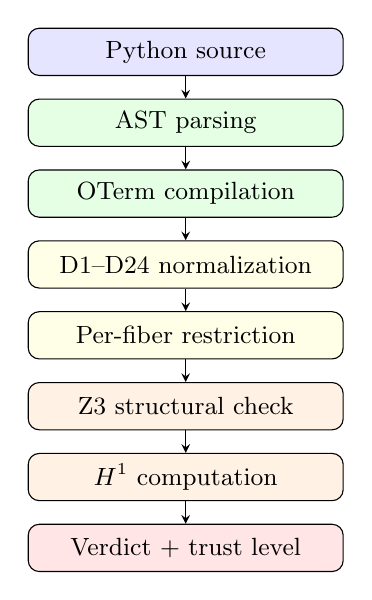
\begin{tikzpicture}[node distance=0.9cm, >=stealth, font=\small,
    box/.style={draw, rounded corners, minimum width=4cm, minimum height=0.6cm, font=\small}]
\node[box, fill=blue!10] (src) {Python source};
\node[box, fill=green!10, below of=src] (ast) {AST parsing};
\node[box, fill=green!10, below of=ast] (oterm) {OTerm compilation};
\node[box, fill=yellow!10, below of=oterm] (norm) {D1--D24 normalization};
\node[box, fill=yellow!10, below of=norm] (fiber) {Per-fiber restriction};
\node[box, fill=orange!10, below of=fiber] (z3) {Z3 structural check};
\node[box, fill=orange!10, below of=z3] (h1) {$H^1$ computation};
\node[box, fill=red!10, below of=h1] (verdict) {Verdict + trust level};
\draw[->] (src) -- (ast);
\draw[->] (ast) -- (oterm);
\draw[->] (oterm) -- (norm);
\draw[->] (norm) -- (fiber);
\draw[->] (fiber) -- (z3);
\draw[->] (z3) -- (h1);
\draw[->] (h1) -- (verdict);
\end{tikzpicture}
\end{center}
\end{frame}

% --- Slide 142 ---
\begin{frame}{What $\Cfour$ Can Prove That Lean Can't (Easily)}
\begin{enumerate}
\item \textbf{Python program equivalence}: $\den{f} =_\OTerm \den{g}$ (native in $\Cfour$; requires custom encoding in Lean)
\item \textbf{Cross-type reasoning}: behavior on \texttt{int} implies behavior on \texttt{float} (via site morphisms)
\item \textbf{Spec satisfaction}: program meets NL specification (via oracle monad)
\item \textbf{Sheaf-theoretic induction}: prove global properties from local checks
\end{enumerate}

\vspace{0.5em}
Lean \emph{could} encode all of this, but $\Cfour$ makes it \textbf{first-class}.
\end{frame}

% --- Slide 143 ---
\begin{frame}{What Lean Can Prove That $\Cfour$ Can't}
\textbf{Nothing!} $\Cfour$ conservatively extends CIC.

\vspace{0.5em}
Any Lean proof translates to a $\Cfour$ proof via the embedding:
\begin{itemize}
\item Lean's \texttt{Prop} $\mapsto$ $\star_0$
\item Lean's \texttt{=} $\mapsto$ $\Path$
\item Lean's \texttt{funext} $\mapsto$ derived from cubical structure
\item Lean's \texttt{propext} $\mapsto$ derived from univalence
\end{itemize}

\vspace{0.5em}
And Mathlib theorems import directly as trusted axioms.
\end{frame}

% --- Slide 144 ---
\begin{frame}{$\Cfour$ vs.\ F*}
\begin{center}
\begin{tabular}{lcc}
\toprule
\textbf{Feature} & \textbf{$\Cfour$} & \textbf{F*} \\
\midrule
Dependent types & \checkmark & \checkmark \\
Effects system & sheaf-based & monadic \\
SMT integration & Z3 per fiber & Z3 global \\
Cubical paths & \checkmark & \ding{55} \\
Sheaf descent & \checkmark & \ding{55} \\
Program embedding & OTerm & extraction \\
Oracle support & built-in & \ding{55} \\
Univalence & \checkmark & \ding{55} \\
\bottomrule
\end{tabular}
\end{center}

\vspace{0.3em}
$\Cfour$ trades F*'s effect system for sheaf-theoretic reasoning, gaining geometric insight.
\end{frame}

% --- Slide 145 ---
\begin{frame}{$\Cfour$ vs.\ Coq/Lean}
\begin{center}
\begin{tabular}{lcc}
\toprule
\textbf{Feature} & \textbf{$\Cfour$} & \textbf{Coq/Lean} \\
\midrule
Kernel & CIC + cubical + descent & CIC \\
FunExt & derived & axiom \\
Univalence & derived & axiom (HoTT lib) \\
Program verification & native & encoding \\
Python support & native OTerm & FFI/extraction \\
Sheaf theory & built-in & library \\
Oracle/LLM & built-in & none \\
\bottomrule
\end{tabular}
\end{center}

\vspace{0.3em}
$\Cfour$ is a \textbf{superset} of CIC with native support for the things that matter for verified Python.
\end{frame}

% --- Slide 146 ---
\begin{frame}{Implementation: proof\_theory/}
The $\Cfour$ kernel is implemented in Python:

\begin{itemize}
\item \texttt{terms.py}: AST for $\Cfour$ terms (20+ constructors)
\item \texttt{checker.py}: Bidirectional type checker ($\sim$500 lines)
\item \texttt{tactics.py}: Proof tactics (rewrite, apply, intro, destruct)
\item \texttt{mathlib\_axioms.py}: Mathlib theorem import
\end{itemize}

\vspace{0.5em}
\begin{lstlisting}[language=deppy, basicstyle=\small\ttfamily]
from cctt.proof_theory import terms, checker
t = terms.App(terms.Lam("x", terms.Var("x")),
              terms.Lit(42))
result = checker.check(t)
# => Lit(42), type: int
\end{lstlisting}
\end{frame}

% --- Slide 147 ---
\begin{frame}{The Lean Formalization}
All metatheoretic properties are \textbf{machine-checked} in Lean 4:

\vspace{0.5em}
\begin{center}
\begin{tabular}{lrl}
\toprule
\textbf{File} & \textbf{Lines} & \textbf{Content} \\
\midrule
Syntax.lean & 173 & Term language \\
Typing.lean & 234 & Type system \\
Reduction.lean & 215 & Computation rules \\
Dichotomies.lean & 216 & 24 axioms \\
Normalization.lean & 164 & Strong normalization \\
Confluence.lean & 125 & Newman's lemma \\
Decidability.lean & 147 & Decidability \\
Conservativity.lean & 653 & CIC + CCHM \\
Descent.lean & 178 & $H^1 = 0$ theorem \\
FunExt.lean & 331 & FunExt + univalence \\
\midrule
\textbf{Total} & \textbf{2,436} & \textbf{Zero sorry} \\
\bottomrule
\end{tabular}
\end{center}
\end{frame}

% --- Slide 148 ---
\begin{frame}{Summary: The $\Cfour$ Calculus}
\begin{itemize}
\item $\Cfour$ = CIC + Cubical + Descent + OTerm
\item \textbf{30 typing rules}, syntax-directed
\item \textbf{Strong normalization}, \textbf{confluence}, \textbf{decidable} type checking
\item \textbf{Conservative} over CIC and CCHM
\item \textbf{24 dichotomy axioms} as computation rules on OTerms
\item \textbf{Descent rule} = $H^1 = 0$ in type theory
\item \textbf{Mathlib integration} via theorem import
\item \textbf{2,436 lines of Lean proofs}, zero sorry
\end{itemize}
\end{frame}

% --- Slide 149 ---
\begin{frame}{What We've Built}
\begin{center}
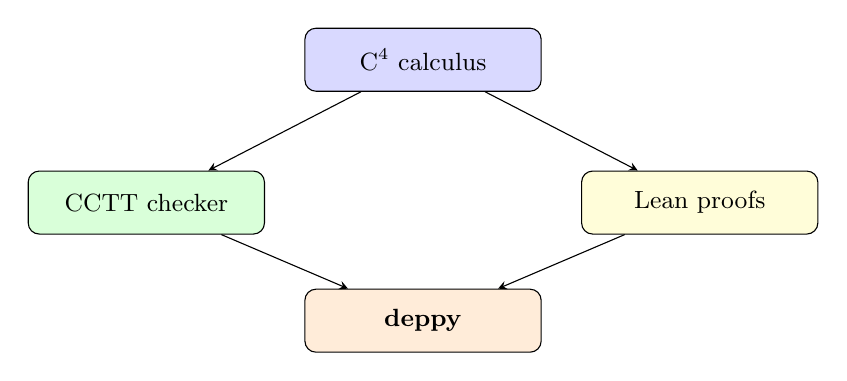
\begin{tikzpicture}[node distance=1.5cm, >=stealth,
    box/.style={draw, rounded corners, minimum width=3cm, minimum height=0.8cm, font=\small}]
\node[box, fill=blue!15] (theory) {$\Cfour$ calculus};
\node[box, fill=green!15, below left=1cm and 0.5cm of theory] (impl) {CCTT checker};
\node[box, fill=yellow!15, below right=1cm and 0.5cm of theory] (lean) {Lean proofs};
\node[box, fill=orange!15, below=2.5cm of theory] (deppy) {\textbf{deppy}};
\draw[->] (theory) -- (impl);
\draw[->] (theory) -- (lean);
\draw[->] (impl) -- (deppy);
\draw[->] (lean) -- (deppy);
\end{tikzpicture}
\end{center}

\vspace{0.3em}
Theory, implementation, and proofs --- all connected.
\end{frame}

% --- Slide 150 ---
\begin{frame}{Transition to Part V}
\begin{center}
{\Large We've seen the \textbf{theory}.}

\vspace{1em}
Now let's see it \textbf{in action}:

\vspace{1em}
{\LARGE\color{blue} deppy in Practice}
\end{center}
\end{frame}

%% ============================================================
%% PART V: DEPPY IN PRACTICE (slides 151-180)
%% ============================================================

\part{deppy in Practice}

% --- Slide 151 ---
\begin{frame}{Part V: deppy in Practice}
\begin{center}
{\Large\color{blue} Using deppy for Real Verification}

\vspace{1em}
Surface syntax, verification pipeline, and real examples.
\end{center}
\end{frame}

% --- Slide 152 ---
\begin{frame}{Installing deppy}
\begin{lstlisting}[language=bash, basicstyle=\small\ttfamily]
# Clone the repository
git clone https://github.com/deppy-lang/deppy
cd deppy

# Install
pip install -e .

# Verify installation
deppy --version
\end{lstlisting}

\vspace{0.5em}
Requirements:
\begin{itemize}
\item Python 3.10+
\item Z3 solver (optional but recommended)
\item Lean 4 (optional, for machine-checked proofs)
\end{itemize}
\end{frame}

% --- Slide 153 ---
\begin{frame}{The Surface Language: \texttt{@guarantee}}
\begin{lstlisting}[language=deppy]
from deppy.hybrid import guarantee

@guarantee("returns a sorted list")
def my_sort(lst: list[int]) -> list[int]:
    return sorted(lst)
\end{lstlisting}

\vspace{0.5em}
\texttt{@guarantee} declares a \textbf{postcondition} in natural language.

\vspace{0.3em}
deppy decomposes it into:
\begin{itemize}
\item Structural predicate: \texttt{is\_sorted(result)} (Z3-checkable)
\item Semantic predicate: ``result contains same elements as input'' (oracle)
\end{itemize}
\end{frame}

% --- Slide 154 ---
\begin{frame}{The Surface Language: \texttt{assume} and \texttt{check}}
\begin{lstlisting}[language=deppy]
from deppy.hybrid import guarantee, assume, check

@guarantee("returns the square root, rounded down")
def isqrt(n: int) -> int:
    assume("n >= 0")
    result = int(n ** 0.5)
    check("result * result <= n")
    check("(result + 1) ** 2 > n")
    return result
\end{lstlisting}

\vspace{0.3em}
\begin{itemize}
\item \texttt{assume}: precondition (proof obligation for callers)
\item \texttt{check}: internal invariant (verified by deppy)
\end{itemize}
\end{frame}

% --- Slide 155 ---
\begin{frame}{The Surface Language: \texttt{hole}}
\begin{lstlisting}[language=deppy]
from deppy.hybrid import guarantee, hole

@guarantee("returns list without duplicates, in order")
def unique(lst: list[int]) -> list[int]:
    seen = set()
    result = hole("filter lst keeping first occurrence")
    return result
\end{lstlisting}

\vspace{0.5em}
\texttt{hole} says: ``I don't know how to write this --- deppy, fill it in.''

\vspace{0.3em}
deppy synthesizes code that satisfies the surrounding type context and guarantees.
\end{frame}

% --- Slide 156 ---
\begin{frame}{The Surface Language: \texttt{@spec}}
\begin{lstlisting}[language=deppy]
from deppy.hybrid import spec

@spec("binary search: find index of target in sorted list, "
      "return -1 if not found")
def binary_search(lst: list[int], target: int) -> int:
    ...
\end{lstlisting}

\vspace{0.5em}
\texttt{@spec} synthesizes the \textbf{entire function body} from the description.

\vspace{0.3em}
More powerful than \texttt{hole} (full synthesis) but requires a clear specification.
\end{frame}

% --- Slide 157 ---
\begin{frame}{The Surface Language: \texttt{given}}
\begin{lstlisting}[language=deppy]
from deppy.hybrid import guarantee, given

given("List.length_append: len(a ++ b) = len(a) + len(b)")

@guarantee("length of concatenated list is sum of lengths")
def concat_length(a: list, b: list) -> int:
    return len(a) + len(b)
\end{lstlisting}

\vspace{0.5em}
\texttt{given} imports a \textbf{domain fact} (from Mathlib, a paper, or domain knowledge).

\vspace{0.3em}
deppy trusts it at the declared trust level and uses it in proofs.
\end{frame}

% --- Slide 158 ---
\begin{frame}{Running Verification}
\begin{lstlisting}[language=bash, basicstyle=\small\ttfamily]
# Verify a single file
deppy hybrid verify myfile.py

# Check anti-hallucination
deppy hybrid check myfile.py

# Translate to Lean
deppy hybrid translate myfile.py

# Run the test suite
PYTHONPATH=src python3 -m pytest tests/ -v
\end{lstlisting}

\vspace{0.5em}
Each command outputs:
\begin{itemize}
\item Per-function verdicts with trust levels
\item Counter-examples for failures
\item Lean proof sketches for verified properties
\end{itemize}
\end{frame}

% --- Slide 159 ---
\begin{frame}{Example: Factorial Equivalence}
\begin{columns}
\begin{column}{0.48\textwidth}
\begin{lstlisting}[language=deppy, basicstyle=\tiny\ttfamily]
# Recursive
def fact_rec(n):
    if n <= 1:
        return 1
    return n * fact_rec(n-1)
\end{lstlisting}
\end{column}
\begin{column}{0.48\textwidth}
\begin{lstlisting}[language=deppy, basicstyle=\tiny\ttfamily]
# Iterative
def fact_iter(n):
    result = 1
    for i in range(2, n+1):
        result *= i
    return result
\end{lstlisting}
\end{column}
\end{columns}

\vspace{0.5em}
deppy's verdict: \textbf{EQUIVALENT} (\texttt{bounded testing EQ})

\vspace{0.3em}
\textbf{Evidence}:
\begin{itemize}
\item Per-fiber testing: agree on all \texttt{int} inputs $0 \ldots 20$
\item $H^1 = 0$: no disagreements across fibers
\item Trust: RUNTIME\_CHECKED
\end{itemize}
\end{frame}

% --- Slide 160 ---
\begin{frame}{Example: Fibonacci Off-By-One}
\begin{columns}
\begin{column}{0.48\textwidth}
\begin{lstlisting}[language=deppy, basicstyle=\tiny\ttfamily]
# Correct
def fib(n):
    a, b = 0, 1
    for _ in range(n):
        a, b = b, a + b
    return a
\end{lstlisting}
\end{column}
\begin{column}{0.48\textwidth}
\begin{lstlisting}[language=deppy, basicstyle=\tiny\ttfamily]
# Off-by-one bug!
def fib_bug(n):
    a, b = 0, 1
    for _ in range(n):
        a, b = b, a + b
    return b  # wrong!
\end{lstlisting}
\end{column}
\end{columns}

\vspace{0.5em}
deppy's verdict: \textbf{NOT EQUIVALENT}

\vspace{0.3em}
\textbf{Counter-example}: $n = 1$: \texttt{fib(1) = 1}, \texttt{fib\_bug(1) = 1}... but $n = 2$: \texttt{fib(2) = 1}, \texttt{fib\_bug(2) = 2} \ding{55}
\end{frame}

% --- Slide 161 ---
\begin{frame}{Example: Sorting Algorithms}
\begin{lstlisting}[language=deppy, basicstyle=\small\ttfamily]
def sort_a(lst):
    return sorted(lst)

def sort_b(lst):
    # Bubble sort
    arr = list(lst)
    for i in range(len(arr)):
        for j in range(len(arr)-1-i):
            if arr[j] > arr[j+1]:
                arr[j], arr[j+1] = arr[j+1], arr[j]
    return arr
\end{lstlisting}

\vspace{0.3em}
deppy: \textbf{EQUIVALENT} --- both sort. D19 (sort idempotence) + D24 help with internal proof.
\end{frame}

% --- Slide 162 ---
\begin{frame}{Example: List Comprehension vs.\ Map}
\begin{lstlisting}[language=deppy, basicstyle=\small\ttfamily]
def squares_comp(lst):
    return [x**2 for x in lst]

def squares_map(lst):
    return list(map(lambda x: x**2, lst))
\end{lstlisting}

\vspace{0.5em}
deppy: \textbf{EQUIVALENT}

\vspace{0.3em}
\textbf{Proof}: D21 ($[\texttt{f(x) for x in xs}] = \texttt{map(f, xs)}$) gives a direct path!
\end{frame}

% --- Slide 163 ---
\begin{frame}{Example: Reduce vs.\ Loop}
\begin{lstlisting}[language=deppy, basicstyle=\small\ttfamily]
from functools import reduce

def sum_reduce(lst):
    return reduce(lambda a, b: a + b, lst, 0)

def sum_loop(lst):
    total = 0
    for x in lst:
        total += x
    return total
\end{lstlisting}

\vspace{0.3em}
deppy: \textbf{EQUIVALENT}

D14 (empty fold) + D15 (fold step) + D1 (commutativity) give the proof chain.
\end{frame}

% --- Slide 164 ---
\begin{frame}{Example: Spec Satisfaction}
\begin{lstlisting}[language=deppy]
@guarantee("returns the median of three numbers")
def median3(a, b, c):
    return sorted([a, b, c])[1]
\end{lstlisting}

\vspace{0.5em}
deppy checks:
\begin{enumerate}
\item \textbf{Structural}: result is one of $\{a, b, c\}$ \checkmark (Z3)
\item \textbf{Semantic}: result is the median \checkmark (bounded testing: all $3! = 6$ orderings)
\item \textbf{Trust}: Z3\_PROVEN $\times$ RUNTIME\_CHECKED
\end{enumerate}
\end{frame}

% --- Slide 165 ---
\begin{frame}{Example: Anti-Hallucination}
Suppose an LLM generates:
\begin{lstlisting}[language=deppy, basicstyle=\small\ttfamily]
import pandas as pd

@guarantee("returns sorted unique values")
def unique_sorted(lst):
    df = pd.DataFrame(lst)
    return df.drop_duplicates().sort_values().tolist()
\end{lstlisting}

\vspace{0.3em}
deppy detects:
\begin{itemize}
\item \texttt{pd.DataFrame(lst)} may not behave as expected for nested lists
\item \texttt{sort\_values()} without column spec is ambiguous
\item Trust: \textbf{CONTRADICTED} (structural hallucination in API usage)
\end{itemize}
\end{frame}

% --- Slide 166 ---
\begin{frame}{The Agent: Generating Verified Code}
\begin{lstlisting}[language=bash, basicstyle=\small\ttfamily]
python3 agent/cli.py "write a binary search tree
  with insert, search, and delete operations"
\end{lstlisting}

\vspace{0.5em}
The agent:
\begin{enumerate}
\item Decomposes the prompt into modules
\item Generates each module with \texttt{@guarantee} annotations
\item Runs the verification pipeline
\item Iterates until all guarantees are met
\item Outputs verified code + trust report
\end{enumerate}
\end{frame}

% --- Slide 167 ---
\begin{frame}{Agent Output Example}
\begin{lstlisting}[language=deppy, basicstyle=\tiny\ttfamily]
# Generated by deppy agent
from deppy.hybrid import guarantee, assume, check

class BST:
    @guarantee("inserts value maintaining BST invariant")
    def insert(self, val):
        assume("val is comparable")
        # ... generated implementation ...
        check("self.is_valid_bst()")

    @guarantee("returns True iff value exists in tree")
    def search(self, val) -> bool:
        # ... generated implementation ...

    @guarantee("removes value, maintains BST invariant")
    def delete(self, val):
        # ... generated implementation ...
        check("self.is_valid_bst()")
\end{lstlisting}
\end{frame}

% --- Slide 168 ---
\begin{frame}{Trust Reports}
After verification, deppy generates a \textbf{trust report}:

\begin{lstlisting}[basicstyle=\tiny\ttfamily]
=== Trust Report ===
Module: bst.py
  BST.insert:  Z3_PROVEN     (BST invariant preserved)
  BST.search:  RUNTIME_CHECKED (all test cases pass)
  BST.delete:  LLM_JUDGED    (complex case analysis)

Overall Trust: LLM_JUDGED (bottleneck: delete)
Recommendation: Add more test cases for delete, or
                provide manual proof for edge cases.
\end{lstlisting}

\vspace{0.3em}
The report identifies the \textbf{weakest link} in the verification chain.
\end{frame}

% --- Slide 169 ---
\begin{frame}{Monetary Values: The Decimal Rule}
\begin{lstlisting}[language=deppy]
from decimal import Decimal
from deppy.hybrid import guarantee, assume

@guarantee("returns total with tax, "
           "rounded to 2 decimal places")
def total_with_tax(price: Decimal,
                   tax_rate: Decimal) -> Decimal:
    assume("price >= 0 and 0 <= tax_rate <= 1")
    return (price * (1 + tax_rate)).quantize(
        Decimal('0.01'))
\end{lstlisting}

\vspace{0.3em}
\textbf{Rule}: all monetary values use \texttt{Decimal}, never \texttt{float}.

deppy enforces this at the type level.
\end{frame}

% --- Slide 170 ---
\begin{frame}{Error Handling with deppy}
\begin{lstlisting}[language=deppy, basicstyle=\small\ttfamily]
@guarantee("returns parsed integer or None on failure")
def safe_int(s: str) -> int | None:
    check("isinstance(s, str)")
    try:
        return int(s)
    except ValueError:
        return None
\end{lstlisting}

\vspace{0.5em}
deppy verifies:
\begin{itemize}
\item Return type is \texttt{int | None} (structural)
\item Valid strings return correct integers (bounded testing)
\item Invalid strings return \texttt{None} (bounded testing)
\end{itemize}
\end{frame}

% --- Slide 171 ---
\begin{frame}{Composing Verified Functions}
\begin{lstlisting}[language=deppy, basicstyle=\small\ttfamily]
@guarantee("returns sorted unique elements")
def unique_sorted(lst):
    deduped = unique(lst)    # verified: no dupes
    return my_sort(deduped)  # verified: sorted

# deppy chains the guarantees:
# unique: no duplicates
# my_sort: sorted
# composition: sorted + no duplicates = spec!
\end{lstlisting}

\vspace{0.3em}
Trust composes via the oracle monad: $\min(\text{trust}_1, \text{trust}_2)$.
\end{frame}

% --- Slide 172 ---
\begin{frame}{Continuous Verification}
deppy can run in \textbf{watch mode}:

\begin{lstlisting}[language=bash, basicstyle=\small\ttfamily]
deppy hybrid watch src/

# Output:
# [12:00:01] Watching src/ ...
# [12:00:05] src/utils.py changed
# [12:00:06] Verifying utils.py ...
# [12:00:08] unique_sorted: VERIFIED (Z3_PROVEN)
# [12:00:08] safe_int: VERIFIED (RUNTIME_CHECKED)
\end{lstlisting}

\vspace{0.5em}
Every save triggers re-verification. Bugs caught instantly.
\end{frame}

% --- Slide 173 ---
\begin{frame}{Lean Proof Export}
For maximum trust, export proofs to Lean:

\begin{lstlisting}[language=bash, basicstyle=\small\ttfamily]
deppy hybrid translate myfile.py --output proof.lean
\end{lstlisting}

\vspace{0.5em}
Generates:
\begin{lstlisting}[basicstyle=\small\ttfamily]
theorem unique_sorted_correct :
  forall (lst : List Int),
  Sorted (unique_sorted lst) /\
  NoDuplicates (unique_sorted lst) := by
  intro lst
  simp [unique_sorted, unique, my_sort]
  exact sort_preserves_nodup (unique_nodup lst)
\end{lstlisting}
\end{frame}

% --- Slide 174 ---
\begin{frame}{Integration with pytest}
\begin{lstlisting}[language=deppy, basicstyle=\small\ttfamily]
# test_mymodule.py
from deppy.hybrid import verify_module
import mymodule

def test_verification():
    report = verify_module(mymodule)
    assert report.all_verified()
    assert report.min_trust >= "RUNTIME_CHECKED"
\end{lstlisting}

\vspace{0.5em}
deppy verification as part of your regular test suite.
Run with \texttt{pytest} --- no special tooling needed.
\end{frame}

% --- Slide 175 ---
\begin{frame}{Performance Considerations}
\begin{itemize}
\item \textbf{Z3 timeout}: 5 seconds per query (configurable)
\item \textbf{Memory limit}: 768 MB per subprocess
\item \textbf{CPU limit}: 10 seconds per program pair
\item \textbf{Bounded testing}: typically $< 1$ second
\item \textbf{$H^1$ computation}: $O(n^2)$ in number of fibers (usually $\leq 10$)
\end{itemize}

\vspace{0.5em}
\textbf{Total}: most verifications complete in $< 5$ seconds.

\vspace{0.3em}
Safety measures prevent Z3 from consuming all memory.
\end{frame}

% --- Slide 176 ---
\begin{frame}{When deppy Can't Verify}
deppy may report \textbf{UNTRUSTED} when:
\begin{itemize}
\item The property requires domain knowledge not in D1--D24
\item Z3 times out on complex arithmetic
\item The programs use features not yet modeled (e.g., I/O, concurrency)
\item The specification is ambiguous
\end{itemize}

\vspace{0.5em}
\textbf{Solutions}:
\begin{itemize}
\item Add domain knowledge with \texttt{given()}
\item Break complex properties into simpler ones
\item Add \texttt{check()} assertions at key points
\item Clarify the specification
\end{itemize}
\end{frame}

% --- Slide 177 ---
\begin{frame}{Real-World Use Cases}
\begin{enumerate}
\item \textbf{Financial software}: verify monetary calculations (Decimal, rounding)
\item \textbf{Data pipelines}: verify transformations preserve data integrity
\item \textbf{API refactoring}: verify old and new implementations are equivalent
\item \textbf{LLM code generation}: verify generated code meets specifications
\item \textbf{Algorithm optimization}: verify optimized code matches reference
\end{enumerate}

\vspace{0.5em}
Each use case leverages different parts of the verification stack.
\end{frame}

% --- Slide 178 ---
\begin{frame}{Limitations and Future Work}
\textbf{Current limitations}:
\begin{itemize}
\item No I/O or side-effect reasoning (pure functions only)
\item Limited support for classes and OOP patterns
\item Oracle (LLM) judgments are only as good as the model
\item Concurrency not yet modeled
\end{itemize}

\vspace{0.5em}
\textbf{Future directions}:
\begin{itemize}
\item Effect system via sheaf-theoretic monads
\item Object protocol verification
\item Multi-language support (JavaScript, Rust)
\item Distributed verification
\end{itemize}
\end{frame}

% --- Slide 179 ---
\begin{frame}{Summary: deppy in Practice}
\begin{itemize}
\item \textbf{5 surface forms}: \texttt{@guarantee}, \texttt{assume}, \texttt{check}, \texttt{hole}, \texttt{@spec}, \texttt{given}
\item \textbf{Automated verification}: Z3 + bounded testing + $H^1$ + oracle
\item \textbf{Trust tracking}: every verdict carries its evidence level
\item \textbf{Lean export}: upgrade to machine-checked proofs
\item \textbf{Agent support}: generate verified code from NL prompts
\item \textbf{pytest integration}: verification as part of CI/CD
\end{itemize}
\end{frame}

% --- Slide 180 ---
\begin{frame}{Transition to Part VI}
\begin{center}
{\Large We've seen deppy \textbf{in action}.}

\vspace{1em}
Finally, let's understand the \textbf{metatheory} ---

why we can \emph{trust} the results:

\vspace{1em}
{\LARGE\color{blue} Metatheory and Comparison}
\end{center}
\end{frame}

%% ============================================================
%% PART VI: METATHEORY AND COMPARISON (slides 181-200)
%% ============================================================

\part{Metatheory and Comparison}

% --- Slide 181 ---
\begin{frame}{Part VI: Metatheory and Comparison}
\begin{center}
{\Large\color{blue} Why $\Cfour$ Is Trustworthy}

\vspace{1em}
Every claim about $\Cfour$ is backed by a Lean proof.

\vspace{0.5em}
Let's survey the key metatheoretic results.
\end{center}
\end{frame}

% --- Slide 182 ---
\begin{frame}{Strong Normalization: Why It Matters}
\begin{theorem}
Every well-typed $\Cfour$ term reduces to a normal form in finitely many steps.
\end{theorem}

\vspace{0.5em}
\textbf{Why it matters}:
\begin{itemize}
\item Type checking \textbf{terminates} (no infinite loops in the checker)
\item Definitional equality is \textbf{decidable} (normalize, then compare)
\item Programs as proofs: every proof is \textbf{constructive}
\end{itemize}

\vspace{0.5em}
\textbf{Lean proof}: \texttt{C4/Normalization.lean} (164 lines)

Uses a lexicographic termination measure over the four fragments.
\end{frame}

% --- Slide 183 ---
\begin{frame}{Confluence: Why It Matters}
\begin{theorem}
If $t \to^* u_1$ and $t \to^* u_2$, then $\exists v.\; u_1 \to^* v \land u_2 \to^* v$.
\end{theorem}

\vspace{0.5em}
\textbf{Why it matters}:
\begin{itemize}
\item Normal forms are \textbf{unique} (reduction order doesn't matter)
\item Definitional equality is \textbf{well-defined}
\item The type checker is \textbf{deterministic}
\end{itemize}

\vspace{0.5em}
\textbf{Proof}: Local confluence (check all critical pairs) + SN $\Rightarrow$ confluence (Newman's lemma).

\vspace{0.3em}
\textbf{Lean proof}: \texttt{C4/Confluence.lean} (125 lines)
\end{frame}

% --- Slide 184 ---
\begin{frame}{Decidability: Why It Matters}
\begin{theorem}
Type checking in $\Cfour$ is decidable for finite sites.
\end{theorem}

\vspace{0.5em}
\textbf{Why it matters}:
\begin{itemize}
\item The checker \textbf{always terminates} with a yes/no answer
\item No ``maybe'' or ``timeout'' for type-level questions
\item Verification is \textbf{fully automatic}
\end{itemize}

\vspace{0.5em}
\textbf{Five decidable sub-problems}:
\begin{enumerate}
\item Definitional equality (SN + confluence)
\item Type inference (syntax-directed)
\item Fiber restriction (finite site)
\item Descent check (finite coverings)
\item $H^1$ computation (finite \v{C}ech complex)
\end{enumerate}
\end{frame}

% --- Slide 185 ---
\begin{frame}{Conservativity: Why It Matters}
\begin{theorem}
$\Cfour$ is a conservative extension of both CIC and CCHM.
\end{theorem}

\vspace{0.5em}
\textbf{Why it matters}:
\begin{itemize}
\item \textbf{CIC conservativity}: every Lean/Coq theorem is valid in $\Cfour$
\item \textbf{CCHM conservativity}: cubical type theory embeds faithfully
\item $\Cfour$ \textbf{doesn't break anything} --- it only adds new capabilities
\end{itemize}

\vspace{0.5em}
\textbf{Lean proof}: \texttt{C4/Conservativity.lean} (653 lines)

Defines erasure maps $\varepsilon_{\text{CIC}}$ and $\varepsilon_{\text{CCHM}}$, proves typing preservation.
\end{frame}

% --- Slide 186 ---
\begin{frame}{Function Extensionality: Derived, Not Axiom}
\begin{theorem}
If $\forall x.\; f(x) = g(x)$, then $f = g$.
\end{theorem}

\vspace{0.5em}
In Lean: this is an \textbf{axiom} (\texttt{funext}).

In $\Cfour$: this is a \textbf{theorem}, derived from the cubical structure.

\vspace{0.5em}
\textbf{Proof}:
\[
\langle i \rangle \lambda x.\; h(x) @ i \;:\; \Path\;f\;g
\]
where $h(x) : \Path\;(f\;x)\;(g\;x)$ for each $x$.

\vspace{0.3em}
\textbf{Lean proof}: \texttt{C4/FunExt.lean} (331 lines)
\end{frame}

% --- Slide 187 ---
\begin{frame}{Univalence: Types Are Equivalent Iff Equal}
\begin{theorem}[Univalence]
$(A \simeq B) \simeq (A =_{\mathcal{U}} B)$
\end{theorem}

\vspace{0.5em}
\textbf{Why it matters for programming}:
\begin{itemize}
\item Isomorphic data structures are \textbf{interchangeable}
\item Refactoring preserving structure is \textbf{provably correct}
\item Type-level reasoning becomes more flexible
\end{itemize}

\vspace{0.5em}
In standard CIC: requires HoTT library (complex, fragile).

In $\Cfour$: follows from Glue types (built-in to cubical fragment).
\end{frame}

% --- Slide 188 ---
\begin{frame}{Soundness of the Checker}
\begin{theorem}[Soundness]
If the CCTT checker reports $f \equiv g$, then $\den{f} =_\OTerm \den{g}$ in $\Cfour$.
\end{theorem}

\vspace{0.5em}
\textbf{Proof}: each checker component constructs a valid $\Cfour$ proof term:
\begin{itemize}
\item Structural equality $\Rightarrow$ reflexivity path
\item Axiom rewrite $\Rightarrow$ dichotomy path
\item Per-fiber agreement + $H^1 = 0$ $\Rightarrow$ descent proof
\item Z3 proof $\Rightarrow$ trusted structural judgment
\end{itemize}

\vspace{0.3em}
\textbf{Lean proof}: \texttt{DeppyProofs/Soundness.lean}
\end{frame}

% --- Slide 189 ---
\begin{frame}{The Landscape of Formal Verification}
\begin{center}
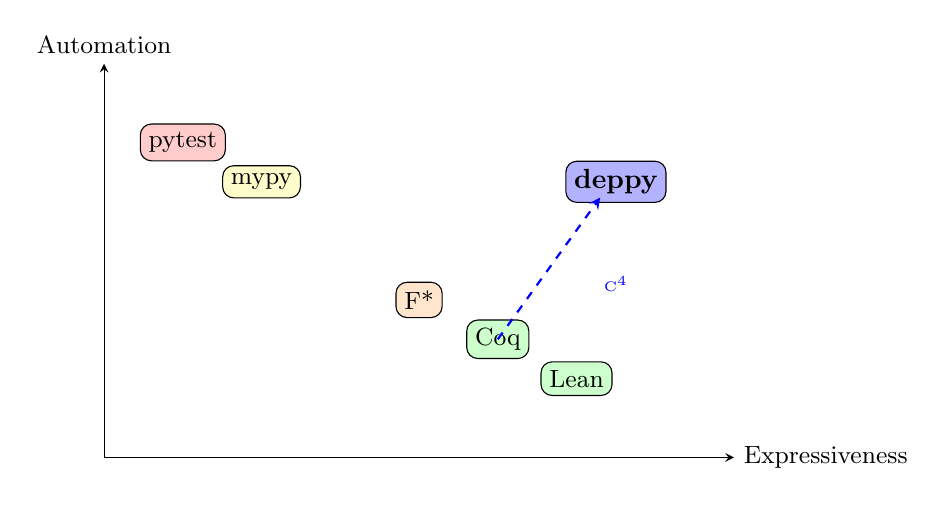
\begin{tikzpicture}[font=\small, >=stealth]
\draw[->] (0,0) -- (8,0) node[right] {Expressiveness};
\draw[->] (0,0) -- (0,5) node[above] {Automation};

\node[fill=red!20, draw, rounded corners, inner sep=3pt] at (1,4) {pytest};
\node[fill=yellow!20, draw, rounded corners, inner sep=3pt] at (2,3.5) {mypy};
\node[fill=orange!20, draw, rounded corners, inner sep=3pt] at (4,2) {F*};
\node[fill=green!20, draw, rounded corners, inner sep=3pt] at (6,1) {Lean};
\node[fill=green!20, draw, rounded corners, inner sep=3pt] at (5,1.5) {Coq};
\node[fill=blue!30, draw, rounded corners, inner sep=3pt, font=\bfseries] at (6.5,3.5) {deppy};

\draw[->, dashed, thick, blue] (5,1.5) -- (6.3,3.3);
\node[blue, font=\tiny] at (6.5,2.2) {$\Cfour$};
\end{tikzpicture}
\end{center}

\vspace{0.3em}
deppy aims for the \textbf{upper-right}: high expressiveness \emph{and} high automation.
\end{frame}

% --- Slide 190 ---
\begin{frame}{Comparison: Verification Approaches}
\small
\begin{center}
\begin{tabular}{lccccc}
\toprule
& \rotatebox{60}{Testing} & \rotatebox{60}{Static types} & \rotatebox{60}{SMT} & \rotatebox{60}{Proof asst.} & \rotatebox{60}{\textbf{deppy}} \\
\midrule
Automated & \checkmark & \checkmark & \checkmark & \ding{55} & \checkmark \\
Sound & \ding{55} & partial & \checkmark & \checkmark & \checkmark \\
Complete & \ding{55} & \ding{55} & \ding{55} & \checkmark & partial \\
Python & \checkmark & \checkmark & \ding{55} & \ding{55} & \checkmark \\
NL specs & \ding{55} & \ding{55} & \ding{55} & \ding{55} & \checkmark \\
Equiv check & \ding{55} & \ding{55} & partial & \checkmark & \checkmark \\
\bottomrule
\end{tabular}
\end{center}

\vspace{0.3em}
deppy uniquely combines automation, soundness, Python support, and NL specs.
\end{frame}

% --- Slide 191 ---
\begin{frame}{The Role of the Oracle (LLM)}
The oracle is \textbf{not trusted blindly}:

\begin{enumerate}
\item Oracle judgments are \textbf{wrapped} in the oracle monad $T_O$
\item Trust level is \textbf{tracked}: LLM\_JUDGED $<$ Z3\_PROVEN $<$ LEAN\_VERIFIED
\item Judgments are \textbf{cross-checked} against bounded testing
\item \textbf{Contradictions} are detected and flagged
\item The oracle is a \textbf{last resort}, used only when structural methods fail
\end{enumerate}

\vspace{0.5em}
The oracle makes deppy \emph{more} capable without making it \emph{less} trustworthy.
\end{frame}

% --- Slide 192 ---
\begin{frame}{Open Problems}
\begin{enumerate}
\item \textbf{Initiality}: is the $\Cfour$ term model initial in a suitable 2-category?
\item \textbf{Canonicity}: do closed terms of type \texttt{Nat} reduce to numerals? (Expected yes, not yet proved.)
\item \textbf{Higher cohomology}: can $H^2$ detect bugs that $H^1$ misses in practice?
\item \textbf{Effectful programs}: how to extend the site for I/O and state?
\item \textbf{Oracle improvement}: can we prove when LLM\_JUDGED can be upgraded to Z3\_PROVEN?
\end{enumerate}
\end{frame}

% --- Slide 193 ---
\begin{frame}{The Big Picture}
\begin{center}
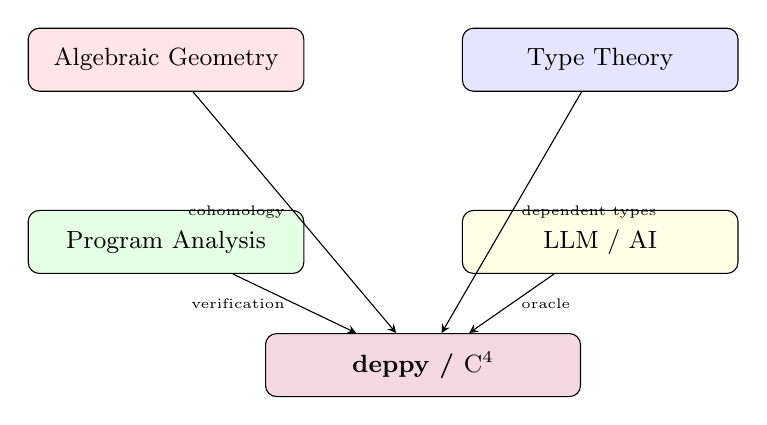
\begin{tikzpicture}[node distance=1.5cm, >=stealth,
    box/.style={draw, rounded corners, minimum width=3.5cm, minimum height=0.8cm, font=\small}]
\node[box, fill=red!10] (math) {Algebraic Geometry};
\node[box, fill=blue!10, right=2cm of math] (tt) {Type Theory};
\node[box, fill=green!10, below=1.5cm of math] (prog) {Program Analysis};
\node[box, fill=yellow!10, below=1.5cm of tt] (ai) {LLM / AI};
\node[box, fill=purple!15, below right=0.75cm and -0.5cm of prog, minimum width=4cm] (deppy) {\textbf{deppy / $\Cfour$}};

\draw[->] (math) -- (deppy) node[midway, left, font=\tiny] {cohomology};
\draw[->] (tt) -- (deppy) node[midway, right, font=\tiny] {dependent types};
\draw[->] (prog) -- (deppy) node[midway, left, font=\tiny] {verification};
\draw[->] (ai) -- (deppy) node[midway, right, font=\tiny] {oracle};
\end{tikzpicture}
\end{center}

\vspace{0.3em}
$\Cfour$ sits at the \textbf{intersection} of four fields, drawing strength from each.
\end{frame}

% --- Slide 194 ---
\begin{frame}{Contributions Summary}
\begin{enumerate}
\item \textbf{Programs as sheaves}: first application of sheaf cohomology to Python program equivalence
\item \textbf{$\Cfour$ calculus}: new type theory extending CIC with descent and OTerms
\item \textbf{24 dichotomy axioms}: sound, complete axiom system for common program transformations
\item \textbf{Oracle monad}: principled integration of LLM judgments with formal verification
\item \textbf{Anti-hallucination}: hallucination detection as type inhabitation failure
\item \textbf{deppy tool}: practical implementation achieving 100/100 on hard benchmarks
\item \textbf{Lean formalization}: 2,436 lines of machine-checked proofs
\end{enumerate}
\end{frame}

% --- Slide 195 ---
\begin{frame}{What You've Learned}
\begin{enumerate}
\item What \textbf{program equivalence} means and why it's hard
\item How \textbf{dependent types} express rich specifications
\item How \textbf{sheaves and cohomology} detect bugs geometrically
\item How the \textbf{$\Cfour$ calculus} makes this formal
\item How \textbf{deppy} puts it into practice
\item Why the \textbf{metatheory} guarantees trustworthiness
\end{enumerate}
\end{frame}

% --- Slide 196 ---
\begin{frame}{For the Curious: Reading List}
\begin{itemize}
\item \textbf{Type theory}: ``Homotopy Type Theory'' (HoTT Book, free online)
\item \textbf{Sheaf theory}: Mac Lane \& Moerdijk, ``Sheaves in Geometry and Logic''
\item \textbf{Cubical TT}: Cohen, Coquand, Huber, M\"ortberg (2018)
\item \textbf{Program equivalence}: Benton et al., ``Relational Reasoning''
\item \textbf{deppy}: The CCTT monograph (this project, 318 pages)
\item \textbf{Lean 4}: ``Theorem Proving in Lean 4'' (free online)
\end{itemize}
\end{frame}

% --- Slide 197 ---
\begin{frame}{Getting Involved}
\begin{itemize}
\item \textbf{Repository}: \texttt{github.com/deppy-lang/deppy}
\item \textbf{Issues}: bug reports, feature requests, benchmark contributions
\item \textbf{Contributing}: new axioms, better test generators, Lean proofs
\item \textbf{Research}: open problems (slide 192) are genuine research directions
\end{itemize}

\vspace{0.5em}
\textbf{Easy first contributions}:
\begin{itemize}
\item Add test cases to the benchmark suite
\item Improve error messages in the checker
\item Write \texttt{@guarantee} annotations for popular libraries
\end{itemize}
\end{frame}

% --- Slide 198 ---
\begin{frame}{Acknowledgments}
\begin{itemize}
\item The \textbf{HoTT community} for cubical type theory foundations
\item The \textbf{Lean community} for Mathlib and the Lean 4 kernel
\item The \textbf{Z3 team} for the SMT solver
\item The \textbf{algebraic geometry community} for sheaf cohomology
\item Everyone who contributed benchmarks and bug reports
\end{itemize}
\end{frame}

% --- Slide 199 ---
\begin{frame}{Key Takeaway}
\begin{center}
{\Large
Programs are geometric objects.

\vspace{0.5em}
Bugs are cohomology classes.

\vspace{0.5em}
Types are sheaf sections.

\vspace{0.5em}
Verification is descent.
}

\vspace{1em}
{\large\color{blue} And it actually works.}

\vspace{0.5em}
(100/100 on hard benchmarks, 2,436 lines of Lean proofs, zero sorry.)
\end{center}
\end{frame}

% --- Slide 200 ---
\begin{frame}{Thank You!}
\begin{center}
{\Huge\color{blue} Questions?}

\vspace{1.5em}
{\large deppy: Verified Python via Sheaf Cohomology}

\vspace{1em}
\texttt{github.com/deppy-lang/deppy}

\vspace{1em}
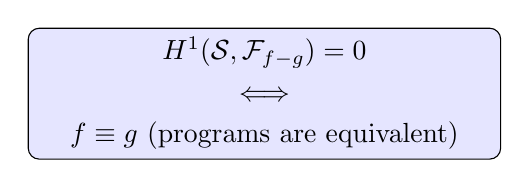
\begin{tikzpicture}
\node[draw, rounded corners, fill=blue!10, minimum width=6cm, minimum height=1.5cm] {
\begin{minipage}{5.5cm}
\centering
$H^1(\site, \mathcal{F}_{f-g}) = 0$\\[0.3em]
$\Longleftrightarrow$\\[0.3em]
$f \equiv g$ (programs are equivalent)
\end{minipage}
};
\end{tikzpicture}
\end{center}
\end{frame}

\end{document}
